\documentclass[11pt,a4paper]{article}
\usepackage[a4paper,margin=25mm]{geometry}
\usepackage[T1]{fontenc}
\usepackage{xcolor,tikz,float}
\usepackage{lmodern,microtype,amsmath,amssymb,amsthm}
\usepackage[pdfusetitle,colorlinks=true,linkcolor=black,citecolor=magenta,urlcolor=black]{hyperref}
\urlstyle{same}
\newtheorem{thm}{Theorem}[section]
\newtheorem{prop}[thm]{Proposition}
\newtheorem{lem}[thm]{Lemma}
\newtheorem{cor}[thm]{Corollary}
\newtheorem{defn}[thm]{Definition}
\newtheorem{conjecture}[thm]{Conjecture}
\newtheorem{introthm}{Theorem}
\renewcommand{\theintrothm}{\Alph{introthm}}
\setlength{\parskip}{1pt}\setlength{\emergencystretch}{2em}
\raggedbottom
\setcounter{tocdepth}{1}

\title{Crossing distances and quantum reflection groups}
\author{Codex, Banica and Claude}
\date{}

\begin{document}
\maketitle
\begin{abstract}
The easy quantum groups $U_N\subset G\subset U_N^+$ of Mang and Weber, coming from pairings whose strings may cross only at certain distances, are indexed by the additive semigroups $D\subset\mathbb N_0$. We associate to each such quantum group $U_N^D$ a quantum reflection group $H_N\subset H_N^{D'}\subset H_N^+$, generated by $H_N$ and by diagonal group duals, coming from reflections placed on the integer line, which commute exactly at the distances in $D$. The correspondence $U_N^D\to H_N^{D'}$ is one-to-one, it reverses inclusions, and $D$ can be recovered from the diagonal tori of either partner. When $0\in D$ the 2 partners generate $U_N^+$, at any $N\geq3$. We also compute the laws of the main characters, which are sums of a Poisson number of reflections, respectively shifted mixed Gaussian variables, and we relate them to each other.
\end{abstract}

\medskip
\noindent {\em Dedicated to Professor R. Speicher, on the occasion of his 67th birthday}
\bigskip

\begingroup
\color{magenta}\hypersetup{linkcolor=magenta}
\setlength{\parskip}{0pt}
\renewcommand{\addvspace}[1]{\vspace{0pt}}
\tableofcontents
\endgroup

\section*{Introduction}
\phantomsection\addcontentsline{toc}{section}{Introduction}

The unitary group $U_N$ and the hyperoctahedral group $H_N$, formed by the signed permutation matrices, have free analogues $U_N^+$ and $H_N^+$, constructed in \cite{bbc,wang}. The liberation question for these groups is that of understanding the intermediate quantum groups
\[
 U_N\subset G\subset U_N^+,\qquad H_N\subset G\subset H_N^+
\]
and in the easy case, where the representation theory of $G$ comes from partitions \cite{bs}, a lot is known. On the unitary side, Mang and Weber constructed in \cite{cyclic,semi} a family of easy quantum groups $U_N^D$, indexed by the additive semigroups $D\subset\mathbb N_0$, with $\mathbb N_0=\{0,1,2,\ldots\}$. On the reflection side, Raum and Weber constructed in \cite{rw,full} easy quantum groups $H_N^\Gamma$, indexed by certain discrete groups $\Gamma$, generated by reflections.

These 2 classifications look quite different. Our aim here is to relate them, by constructing a correspondence as follows, where $D'$ is a reflection group, depending on $D$:
\[
 U_N^D\quad\longrightarrow\quad H_N^{D'}.
\]

Let us first explain what $U_N^D$ is. The fixed vectors of $U_N^+$, in the various tensor products between the fundamental representation $u$ and its conjugate $\bar u$, come from the noncrossing pairings of a row of points, colored white for $u$ and black for $\bar u$. Read the row as a walk on the integers, with a step up at each white point, and a step down at each black point. Each string of our pairing joins an upward step and a downward step along the same edge $\{h,h+1\}$ of the integer line, and we call $h$ the height of the string.

Now let us allow crossings. For an additive semigroup $D\subset\mathbb N_0$, the fixed vectors of $U_N^D$ come by definition from the pairings as above, where 2 strings $P,Q$ are allowed to cross only when the difference between their heights lies outside $D$:
\[
 P,Q\ \text{cross}\implies|height(P)-height(Q)|\notin D.
\]

Thus, $D$ is the set of forbidden crossing distances. With $D=\mathbb N_0$ nothing may cross, and we get $U_N^+$. When $D$ gets smaller there are more fixed vectors, and so $U_N^D$ gets smaller.

On the reflection side, we use the same integer line. Assume first $0\in D$. We put a reflection $s_i$ at each integer $i$, and we let $W_D$ be the group generated by these reflections, with the relations $s_i^2=1$, and with the following commutation relations:
\[
 s_is_j=s_js_i\qquad\text{when }|i-j|\in D.
\]
There are no other relations, so $s_i,s_j$ are free when $|i-j|\notin D$. When $0\notin D$ we put 2 free reflections $s_i,s_i'$ at each integer $i$, with the same rule for reflections at different integers. Now choose $N$ of our reflections $r_1,\ldots,r_N$, with repetitions allowed. The group $\langle r_1,\ldots,r_N\rangle$ has a dual, which is a quantum subgroup of $H_N^+$, with fundamental representation $diag(r_1,\ldots,r_N)$. We define $H_N^{D'}$ to be the quantum subgroup of $H_N^+$ generated by $H_N$, and by all these group duals:
\[
 H_N^{D'}=\Big\langle H_N,\ \widehat{\langle r_1,\ldots,r_N\rangle}\Big\rangle.
\]

As for the group $D'$ itself, this has generators $g_1,g_2,\ldots$ of order 2, and a word in these generators is a relation when it holds for commuting signs, and for any choice of reflections $r_1,r_2,\ldots$ as above. We will see that $D'$ is one of the groups from \cite{rw}, so $H_N^{D'}$ is easy.

In order to see where the correspondence comes from, consider the diagonal torus of $U_N^D$, obtained by setting the off-diagonal entries of $u$ equal to $0$. With $a,b$ being the first 2 diagonal entries, the elements $x_i=a^i(ba^{-1})a^{-i}$ generate, together with $a$, the dual of the torus at $N=2$, and the only relations between them are commutation relations. To be more precise, at $i\neq j$ the rules on the 2 sides are as follows:
\[
 x_ix_j=x_jx_i\iff|i-j|\notin D,\qquad\quad s_is_j=s_js_i\iff|i-j|\in D.
\]

Thus, what commutes on the unitary side is free on the reflection side, and vice versa. As an illustration, $D=\mathbb N_0$ corresponds to $U_N^+$, whose torus is a free group dual, and the reflection partner comes from commuting reflections, and is $H_N$. At the other end, $D=\{0\}$ gives free reflections, and the reflection partner is $H_N^{[\infty]}$, the largest group-theoretical easy quantum reflection group from \cite{rw,full}. The general picture is as follows:

\begin{figure}[H]
\centering
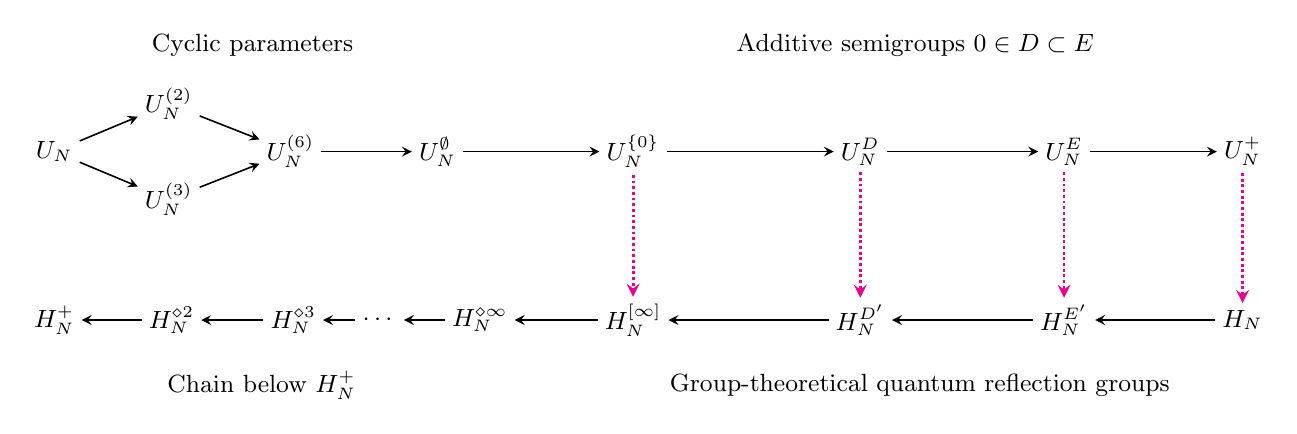
\begin{tikzpicture}[x=1.145cm,y=1.38cm,>=stealth,inner sep=2.3pt,line width=.58pt,font=\small]
\node at (2.2,2.48) {Cyclic parameters};
\node at (9.55,2.48) {Additive semigroups $0\in D\subset E$};
\node (u) at (0,1.50) {$U_N$};
\node (u2) at (1.27,1.94) {$U_N^{(2)}$};
\node (u3) at (1.27,1.06) {$U_N^{(3)}$};
\node (u6) at (2.62,1.50) {$U_N^{(6)}$};
\node (empty) at (4.25,1.50) {$U_N^{\emptyset}$};
\node (zero) at (6.42,1.50) {$U_N^{\{0\}}$};
\node (ud) at (8.94,1.50) {$U_N^D$};
\node (ue) at (11.20,1.50) {$U_N^E$};
\node (up) at (13.18,1.50) {$U_N^+$};
\foreach \a/\b in {u/u2,u/u3,u2/u6,u3/u6,u6/empty,empty/zero,zero/ud,ud/ue,ue/up}
  \draw[->] (\a) -- (\b);
\node (hp) at (0,-.05) {$H_N^+$};
\node (l2) at (1.30,-.05) {$H_N^{\diamond 2}$};
\node (l3) at (2.65,-.05) {$H_N^{\diamond 3}$};
\node (dots) at (3.61,-.05) {$\cdots$};
\node (linf) at (4.72,-.05) {$H_N^{\diamond\infty}$};
\node (free) at (6.42,-.05) {$H_N^{[\infty]}$};
\node (hd) at (8.94,-.05) {$H_N^{D'}$};
\node (he) at (11.20,-.05) {$H_N^{E'}$};
\node (h) at (13.18,-.05) {$H_N$};
\foreach \a/\b in {l2/hp,l3/l2,dots/l3,linf/dots,free/linf,hd/free,he/hd,h/he}
  \draw[->] (\a) -- (\b);
\foreach \a/\b in {zero/free,ud/hd,ue/he,up/h}
  \draw[->,densely dotted,magenta,line width=1.05pt] (\a.south) -- (\b.north);
\node at (2.30,-.65) {Chain below $H_N^+$};
\node at (9.60,-.65) {Group-theoretical quantum reflection groups};
\end{tikzpicture}
\caption{The dotted arrows give the correspondence, on the branch $0\in D$. The solid arrows are inclusions. An inclusion on the upper right reverses direction on the lower right.}
\label{classification}
\end{figure}

Here on the left we have the remaining easy quantum groups from \cite{cyclic,full}, which are not concerned by our correspondence. The point indeed is that the full easy liberation intervals of $U_N$ and $H_N$ cannot be matched, as we will see in Section~\ref{unitary}.

In order to state our first result, we need a description of the image. Assume that $D$ has positive elements, and let $d$ be their greatest common divisor. Then $D\cup\{0\}=dS$, where $S$ is an additive semigroup containing $0$, whose complement $B=\mathbb N_0-S$ is finite. Finally, set $t=1$ when $0\in D$, and $t=2$ otherwise. Thus $t$ is the number of reflections at each integer.

\begin{introthm}\label{intro-image}
The correspondence $U^D\to H^{D'}$ is one-to-one, with $D$ ranging over the nonempty additive semigroups of $\mathbb N_0$, and with the quantum groups being compared in all dimensions $N$. It reverses inclusions, in the sense that for $D\subset E$ we have
\[
 U_N^D\subset U_N^E,\qquad H_N^{E'}\subset H_N^{D'}
\]
at any $N$. Its image consists of $H^{[\infty]}$, and of one quantum reflection group for each triple $(d,B,t)$, where $d\geq1$, $t=1,2$, and $B$ is a finite set of positive integers such that $\mathbb N_0-B$ is an additive semigroup.
\end{introthm}

The proof of the injectivity is the most technical part of the paper. The problem is that when looking at $H_N^{D'}$ the reflections $s_i$ no longer carry their integer labels, and these labels must be reconstructed, from the diagonal group dual subgroups of $H_N^{D'}$.

How can we find the partner, if we are given just the unitary quantum group? As already said, the answer comes from the diagonal torus. At $N=2$ this torus only sees the positive distances. With one more coordinate we can test the distance $0$ as well.

\begin{introthm}\label{intro-torus}
Let $D\subset\mathbb N_0$ be a nonempty additive semigroup, let $a,b,c$ be the standard coordinates of the diagonal torus of $U_3^D$, and set $x=ba^{-1}$, $y=ca^{-1}$. Then
\[
 x\,(a^kya^{-k})=(a^kya^{-k})\,x\iff k\notin D
\]
for any $k\in\mathbb N_0$. In particular these $3$ coordinates determine $D$.
\end{introthm}

As a basic example, take $D_*=\{0,2,3,4,\ldots\}$. This is the largest additive semigroup containing $0$, apart from $\mathbb N_0$ itself, and the only allowed crossing distance is $1$. On the reflection side the commutation relations are $s_is_j=s_js_i$ for $|i-j|\geq2$. Thus the reflections form a path, with neighbors being free:

\begin{figure}[H]
\centering
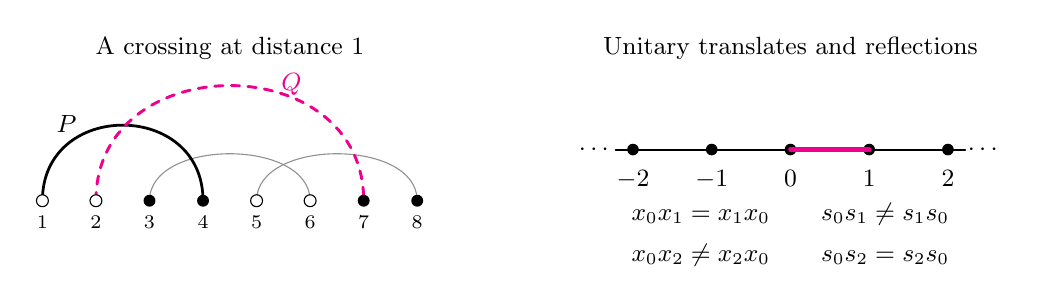
\begin{tikzpicture}[x=1cm,y=1cm,line cap=round,line join=round,font=\small]
\begin{scope}[x=.68cm]
\node at (3.5,1.94) {A crossing at distance $1$};
\draw[black!43] (2,0) to[out=90,in=90] (5,0);
\draw[black!43] (4,0) to[out=90,in=90] (7,0);
\draw[line width=1pt] (0,0) .. controls (0,1.28) and (3,1.28) .. (3,0);
\draw[magenta,line width=1.05pt,dashed] (1,0) .. controls (1,1.95) and (6,1.95) .. (6,0);
\node at (.45,.98) {$P$};
\node[magenta] at (4.65,1.48) {$Q$};
\foreach \j in {0,1,4,5} \draw[fill=white] (\j,0) circle[radius=2.15pt];
\foreach \j in {2,3,6,7} \fill (\j,0) circle[radius=2.15pt];
\foreach \j in {0,...,7} \node[below=2pt,font=\scriptsize] at (\j,0) {\the\numexpr\j+1\relax};
\end{scope}
\begin{scope}[shift={(9.5,0)}]
\node at (0,1.94) {Unitary translates and reflections};
\draw[line width=.7pt] (-2.22,.65)--(2.22,.65);
\foreach \j in {-2,...,2} {
  \fill (\j,.65) circle[radius=2.1pt];
  \node[below=4pt] at (\j,.65) {$\j$};
}
\node at (-2.47,.65) {$\cdots$};
\node at (2.47,.65) {$\cdots$};
\draw[magenta,line width=1.65pt] (0,.65)--(1,.65);
\node at (0,-.17) {$x_0x_1=x_1x_0\qquad s_0s_1\ne s_1s_0$};
\node at (0,-.69) {$x_0x_2\ne x_2x_0\qquad s_0s_2=s_2s_0$};
\end{scope}
\end{tikzpicture}
\caption{The parameter $D_*$. On the left the walk goes up twice, down twice, and then again. The string $P$ has height $0$, the string $Q$ has height $1$, and they are allowed to cross. On the right, the integers which are joined carry free reflections.}
\label{gap-picture}
\end{figure}

On this path any 2 neighbors are free, but among 3 reflections at least 2 commute, or coincide. Thus the reflection partner of $U_N^{D_*}$ has free diagonal entries, exactly as $H_N^{[\infty]}$, at $N=2$, but no longer at $N=3$. Here is the general statement, of this type:

\begin{introthm}\label{intro-embedding}
For $D=\{0\}$ we have $H_N^{D'}=H_N^{[\infty]}$, in any dimension. Otherwise, with $m$ being the smallest positive element of $D$, and with $t=1,2$ being as above, we have
\[
 H_N^{D'}=H_N^{[\infty]}\iff N\leq tm
\]
with the equality on the left meaning that the diagonal entries of $H_N^{D'}$ are free.
\end{introthm}

At the other extreme, when $1\in D$ all the positive distances are in $D$, and the reflections at different integers commute. In this case we only keep the reflections at $0$. We obtain in this way the group $H_N$, and the half-liberation $H_N^*$ of it, as partners of the quantum groups $U_N^+$ and $U_N^\times$, with this latter quantum group being given by the relations $uv^*w=wv^*u$:

\begin{figure}[H]
\centering
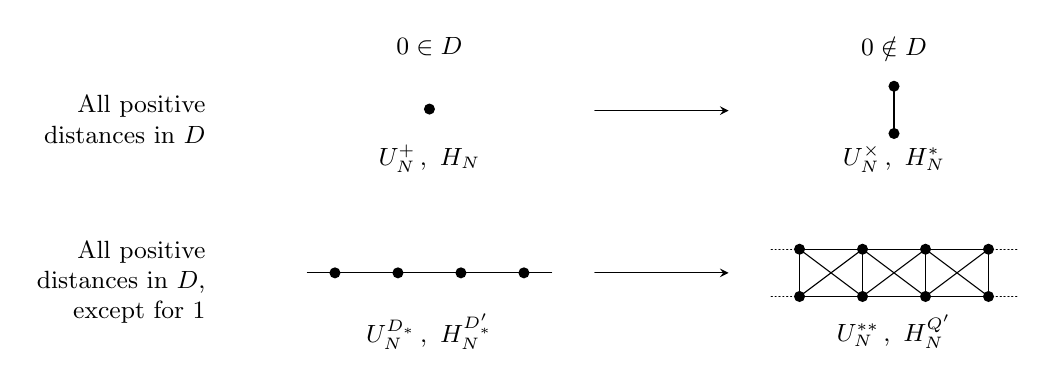
\begin{tikzpicture}[x=1cm,y=1cm,font=\small,line cap=round,line join=round]
\node at (2.6,1.45) {$0\in D$};
\node at (8.5,1.45) {$0\notin D$};
\node[anchor=east,align=right] at (-.12,.53) {All positive\\distances in $D$};
\node[anchor=east,align=right] at (-.12,-1.54) {All positive\\distances in $D$,\\except for $1$};
\fill (2.6,.66) circle (2pt);
\node at (2.6,.03) {$U_N^+\,,\ H_N$};
\draw[thick] (8.5,.35)--(8.5,.95);
\foreach \y in {.35,.95} \fill (8.5,\y) circle (2pt);
\node at (8.5,.03) {$U_N^\times\,,\ H_N^*$};
\foreach \x in {1.4,2.2,3,3.8} \fill (\x,-1.42) circle (2pt);
\draw (1.05,-1.42)--(4.15,-1.42);
\node at (2.6,-2.17) {$U_N^{D_*}\,,\ H_N^{D_*'}$};
\foreach \x in {7.3,8.1,8.9,9.7}{
  \draw (\x,-1.12)--(\x,-1.72);
  \foreach \y in {-1.12,-1.72} \fill (\x,\y) circle (2pt);
}
\foreach \x in {7.3,8.1,8.9}{
  \foreach \y in {-1.12,-1.72}
    \foreach \z in {-1.12,-1.72} \draw (\x,\y)--({\x+.8},\z);
}
\foreach \y in {-1.12,-1.72}{\draw[densely dotted] (6.94,\y)--(7.3,\y) (9.7,\y)--(10.06,\y);}
\node at (8.5,-2.17) {$U_N^{**}\,,\ H_N^{Q'}$};
\draw[->,>=stealth] (4.7,.64)--(6.4,.64);
\draw[->,>=stealth] (4.7,-1.42)--(6.4,-1.42);
\end{tikzpicture}
\caption{Removing $0$ from $D$ doubles each reflection. The reflections which are joined are free, and the other ones commute. On the right we have the partners of the unitary half-liberations $U_N^\times,U_N^{**}$ from \cite{semi}, with $Q=\{2,3,4,\ldots\}$.}
\label{double-picture}
\end{figure}

Let us put now both partners inside the same quantum group, namely $U_N^+$. For the path, the reflection partner contains the dual of $\mathbb Z_2*\mathbb Z_2$, acting on a coordinate plane. This turns out to be exactly what is missing from the unitary partner, in order to generate $U_N^+$:

\begin{introthm}\label{intro-joint}
Let $D\subset\mathbb N_0$ be an additive semigroup containing $0$. We have then
\[
 \big\langle U_N^D,H_N^{D'}\big\rangle=U_N^+
\]
for any $N\geq3$. In fact, when $D\neq\mathbb N_0$, it suffices to adjoin to $U_N^D$ the diagonal subgroup with $2$ free reflections on a coordinate plane, and the identity on its complement. At $N=2$ the reflection partner is contained in $U_2^D$.
\end{introthm}

Another way of comparing the partners is by looking at the main character $\chi=\sum_iu_{ii}$, whose moments with respect to the Haar integration count the fixed vectors \cite{bs,wor}. For $H_N^{D'}$ we obtain with $N\to\infty$ a sum $Y_D=g_1+\ldots+g_f$ of generators of $D'$, with $f$ being an independent Poisson variable. For $U_N^D$ we obtain a variable of type $Z_D=c_0v$, with $c_0$ being Gaussian, part of a family of Gaussian variables $c_i$ indexed by the integers, which mix classical and free independence, according to $D$, and with $v$ being the shift of the integers. The simplest relation between these variables is as follows:

\begin{introthm}\label{intro-seven}
For the limiting main characters $Z_D$ of $U_N^D$ and $Y_D$ of $H_N^{D'}$ we have
\[
 \tau\!\left[\bigl(Z_D^2(Z_D^*)^2\bigr)^2\right]+\tau(Y_D^4)=7
\]
for any additive semigroup $D\subset\mathbb N_0$ containing $0$, with $\tau$ being the expectation.
\end{introthm}

Here the point is that the distance $1$ is seen by both quantities. For the path $D_*$ the sum reads $4+3$, while for $D=\mathbb N_0$, where we have $U_N^+$ and $H_N$, the sum reads $3+4$.

At the level of the higher moments, the natural object is the order on the integers given by $i\preceq j$ when $j-i\in D$. Indeed, the reflections $s_i,s_j$ commute when $i,j$ are comparable, and are free otherwise. On the unitary side we have the following result, where $NC(p)$ is the lattice of noncrossing partitions of $\{1,\ldots,p\}$:

\begin{introthm}\label{intro-order}
Let $D\subset\mathbb N_0$ be an additive semigroup containing $0$. For any $k,p\geq1$, the number
\[
 \tau\!\left[\bigl(Z_D^k(Z_D^*)^k\bigr)^p\right]
\]
equals the number of maps $\{0,\ldots,k-1\}\to NC(p)$ which are increasing with respect to $\preceq$. At $p=2$ and $D\neq\mathbb N_0$ this is the number of subsets of $\{s_0,\ldots,s_{k-1}\}$ consisting of pairwise free reflections.
\end{introthm}

This contains for instance the fact that for $U_N^+$ we get the Fuss--Catalan numbers, and for the smallest parameter $D=\{0\}$ we get powers of Catalan numbers. Also, these moments determine $D$. On the reflection side the situation is more subtle. We will show that the first moment distinguishing between the path partner and $H_N^{[\infty]}$ is the 30th one, and that in fact, apart from $H_N,H_N^*$, all the partners have the same moments up to order 29.

We also discuss the first dimension $N$ where 2 given reflection partners $H_N^{D'},H_N^{E'}$ become different, with exact results in several cases, an explicit bound in general, and a conjecture, verified by computer for small parameters. Finally, several questions are left open.

The paper is organized as follows. Section~\ref{unitary} contains preliminaries on $U_N^D$. In Sections~\ref{tori} and~\ref{reflection} we compute the diagonal tori of $U_N^D$, and we construct the reflection partners. In Sections~\ref{detection} and~\ref{recover} we recover $D$ from the reflection partner, and we describe the image. Sections~\ref{examples} and~\ref{separation} contain the dimension results, and the half-liberations. In Section~\ref{joint-section} we discuss what the partners generate together. In Sections~\ref{reflection-laws} and~\ref{unitary-laws} we compute the character laws, and in Section~\ref{paired-laws} we compare them.

\section{Crossing distances and easiness}\label{unitary}

We use the compact matrix quantum group formalism of Woronowicz \cite{wor}. The free unitary quantum group $U_N^+$ was constructed by Wang in \cite{wang}. Its algebra $C(U_N^+)$ is the universal $C^*$-algebra generated by the entries of a $N\times N$ matrix $u=(u_{ij})$, subject to the relations stating that both $u$ and $\bar u=(u_{ij}^*)$ are unitaries. As for the quantum reflection group $H_N^+$ from \cite{bbc}, this is the closed subgroup $H_N^+\subset U_N^+$ obtained by further imposing the following relations, which state that the entries $u_{ij}$ are self-adjoint, and that on each row and column of $u$, the distinct entries have products $0$:
\[
 u_{ij}=u_{ij}^*,\qquad u_{ij}u_{ik}=u_{ji}u_{ki}=0\quad(j\neq k).
\]

Here, and in what follows, the closed subgroups $G\subset U_N^+$ correspond to the quotients $C(U_N^+)\to C(G)$ which are compatible with the comultiplication, counit and antipode.

We will need 3 basic constructions. First, any discrete group $\Gamma=\langle g_1,\ldots,g_N\rangle$ produces a closed subgroup $\widehat\Gamma\subset U_N^+$, called group dual, with $C(\widehat\Gamma)=C^*(\Gamma)$ and with fundamental representation $u=diag(g_1,\ldots,g_N)$. Second, any closed subgroup $G\subset U_N^+$ has a diagonal torus, obtained by setting $u_{ij}=0$ for $i\neq j$. This is a group dual, and is the largest group dual inside $G$ having a diagonal fundamental representation. Finally, given $G,H\subset U_N^+$, we denote by $\langle G,H\rangle$ the smallest closed subgroup of $U_N^+$ containing both of them. See \cite{bcf,chir}.

Let us discuss now easiness. Consider a row of $k$ points, colored white or black. With the conventions $u^\circ=u$ and $u^\bullet=\bar u$, we can associate to this row $\alpha=\alpha_1\ldots\alpha_k$ the following tensor product representation, on the space $(\mathbb C^N)^{\otimes k}$:
\[
 u^{\otimes\alpha}=u^{\alpha_1}\otimes\ldots\otimes u^{\alpha_k}.
\]

By Tannakian duality \cite{wor}, a closed subgroup $G\subset U_N^+$ is uniquely determined by the spaces $Fix(u^{\otimes\alpha})$ of fixed vectors of these representations. Now let $\pi$ be a pairing of our $k$ points. With $e_1,\ldots,e_N$ being the standard basis of $\mathbb C^N$, we can associate to it the vector
\[
 \xi_\pi=\sum_{i_1,\ldots,i_k}\delta_\pi(i_1,\ldots,i_k)\,e_{i_1}\otimes\ldots\otimes e_{i_k}
\]
where $\delta_\pi=1$ when the indices are equal on each string of $\pi$, and $\delta_\pi=0$ otherwise. A closed subgroup $G\subset U_N^+$ is called easy when its spaces $Fix(u^{\otimes\alpha})$ are spanned by such vectors $\xi_\pi$, with $\pi$ belonging to certain sets of partitions $P(\alpha)$, which must form a category in the sense of \cite{bs,tw}. Here we will only need pairings. For $U_N^+$ itself the fixed vectors come from the noncrossing pairings which join white points to black points \cite{bs,tw}.

In order to introduce the quantum groups $U_N^D$, read the row $\alpha$ as a walk on the integers, starting at $0$, with a step up at each white point, and a step down at each black point. The step number $j$ runs along a certain edge $\{h,h+1\}$ of the integer line, and we call $h$ the height of the point $j$. Here is an example, with the points having heights $0,1,1,0,0,1,1,0$:

\begin{figure}[H]\centering
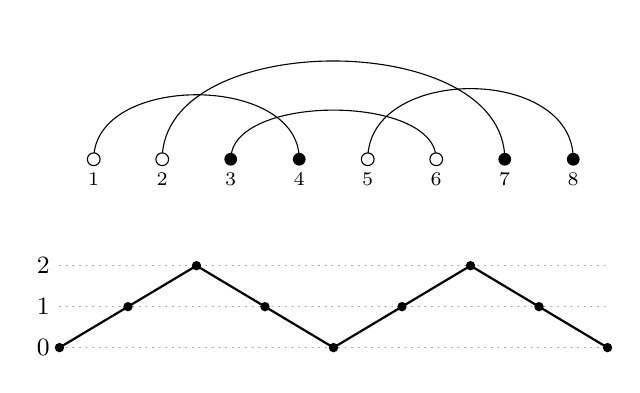
\begin{tikzpicture}[x=.87cm,y=.52cm,line cap=round]
\foreach \i/\j/\h in {1/4/2.1,2/7/3.2,3/6/1.6,5/8/2.3}
 \draw (\i,0) .. controls (\i,\h) and (\j,\h) .. (\j,0);
\foreach \i in {1,2,5,6}\draw[fill=white] (\i,0) circle (2.3pt);
\foreach \i in {3,4,7,8}\fill (\i,0) circle (2.3pt);
\foreach \i in {1,...,8}\node[below,font=\scriptsize] at (\i,-.1) {$\i$};
\begin{scope}[shift={(.5,-4.6)}]
\foreach \y in {0,1,2}{\draw[black!35,dotted] (0,\y)--(8,\y);\node[left,font=\small] at (0,\y){$\y$};}
\draw[thick] (0,0)--(1,1)--(2,2)--(3,1)--(4,0)--(5,1)--(6,2)--(7,1)--(8,0);
\foreach \x/\y in {0/0,1/1,2/2,3/1,4/0,5/1,6/2,7/1,8/0}\fill (\x,\y) circle(1.7pt);
\end{scope}
\end{tikzpicture}
\caption{A row of 8 points, with its walk below, and a pairing of it. The point $i$ is right above the step $i$ of the walk. The strings $(1,4)$ and $(5,8)$ have height $0$, and the strings $(2,7)$ and $(3,6)$ have height $1$. Each string of height $0$ crosses each string of height $1$.}
\label{pairing-walk}
\end{figure}

We are interested in the pairings whose strings can be given a height, as in the above picture. This leads to the following notions:

\begin{defn}\label{horizontal}
A pairing of a colored row is called horizontal when each of its strings joins $2$ points of different colors, having the same height. The common height of the $2$ points is called height of the string, and the distance between $2$ strings is
\[
 d(P,Q)=|height(P)-height(Q)|
\]
which is an element of $\mathbb N_0$.
\end{defn}

Equivalently, each string must join a white point and a black point, and between these 2 points there must be as many white points as black points. This is the formulation from \cite{semi}. We agree as usual that 2 strings $(p,q)$ and $(p',q')$ cross when their endpoints alternate, in the sense that $p<p'<q<q'$, or $p'<p<q'<q$.

\begin{defn}\label{unitary-def}
Given an additive semigroup $D\subset\mathbb N_0$, possibly empty, we denote by $I_D(\alpha)$ the set of horizontal pairings $\pi$ of the row $\alpha$ having the property
\[
 P,Q\in\pi\ \text{cross}\implies d(P,Q)\notin D
\]
for any $2$ strings $P,Q$. Thus, $D$ is the set of forbidden crossing distances.
\end{defn}

In the above picture all the crossings have distance $1$. Thus, the pairing there belongs to $I_D$ precisely when $1\notin D$. The following result is due to Mang and Weber:

\begin{thm}[\cite{semi}]\label{mang-weber}
For any additive semigroup $D\subset\mathbb N_0$, possibly empty, there is an easy quantum group $U_N\subset U_N^D\subset U_N^+$ whose spaces of fixed vectors are
\[
 Fix(u^{\otimes\alpha})=span\big(\xi_\pi\,\big|\,\pi\in I_D(\alpha)\big)
\]
for any colored row $\alpha$. Moreover, we have $U_N^D\subset U_N^E$ whenever $D\subset E$.
\end{thm}

Observe that the last assertion is clear, because enlarging $D$ removes pairings, and so removes fixed vectors. As a first example, at $D=\mathbb N_0$ no crossing is allowed, and we obtain $U_N^+$. With $K=\{1,2,3,\ldots\}$ the only crossings are those at distance $0$, and we obtain the quantum group $U_N^\times$, given by the relations $uv^*w=wv^*u$, between the entries of the fundamental representation. With $Q=\{2,3,4,\ldots\}$ we obtain the quantum group $U_N^{**}$, where the products $uv^*,u^*v$ all commute with each other. See \cite{semi}. Our main example will be
\[
 D_*=\{0,2,3,4,\ldots\}
\]
where the crossings must have distance exactly $1$, as in Figure~\ref{pairing-walk}. Finally, at $D=\emptyset$ all the horizontal pairings are allowed. According to the classification results in \cite{cyclic,semi}, the quantum groups $U^D$ with $D\neq\emptyset$ are precisely the easy quantum groups $U^\emptyset\subsetneq G\subset U^+$.

We will need the fact that each allowed crossing distance really occurs:

\begin{lem}\label{crossing-exists}
For any $k\in\mathbb N_0$ with $k\notin D$ there is a colored row $\alpha$ and a pairing $\pi\in I_D(\alpha)$ having $2$ crossing strings, of heights $0$ and $k$.
\end{lem}

\begin{proof}
At $k=0$ we can take the row $\circ\bullet\circ\bullet\circ\bullet$, whose points all have height $0$, with the pairing $(1,4),(2,5),(3,6)$, whose strings all cross. At $k\geq1$ take the row $(\circ^{k+1}\bullet^{k+1})^2$. The walk goes up to $k+1$ and back to $0$, twice. Each edge $\{i,i+1\}$ with $0\leq i\leq k$ is run through 4 times, at certain points $u_i<v_i<u_i'<v_i'$ of colors $\circ,\bullet,\circ,\bullet$, and for $i<j$ we have
\[
 u_i<u_j<v_j<v_i<u_i'<u_j'<v_j'<v_i'.
\]

At each height $i$ there are 2 ways of joining these points, namely
\[
 P_i=\{(u_i,v_i),(u_i',v_i')\},\qquad Q_i=\{(u_i,v_i'),(v_i,u_i')\}.
\]

From the above inequalities we see that, at $i<j$, the strings at height $i$ cross those at height $j$ precisely when we choose $P_i$ and $Q_j$. Now choose $Q_j$ when $k-j\in D\cup\{0\}$, and $P_j$ otherwise. If we have $P_i$ and $Q_j$ with $i<j$ then $j-i\notin D$, because otherwise the number
\[
 k-i=(k-j)+(j-i)
\]
would belong to $D$, and we would have $Q_i$. Thus our pairing is in $I_D$. Finally, we have $P_0$ and $Q_k$, due to $k\notin D$, so the strings at heights $0$ and $k$ cross.
\end{proof}

As a first consequence, the parameter $D$ is uniquely determined by the quantum groups $U_N^D$, taken altogether. More precisely, we have the following result:

\begin{prop}\label{order-unitary}
For additive semigroups $D,E\subset\mathbb N_0$ we have $D\subset E$ if and only if $U_N^D\subset U_N^E$ for any $N$.
\end{prop}

\begin{proof}
One implication is known from Theorem~\ref{mang-weber}. Conversely, assume $k\in D$, $k\notin E$, and let $\pi\in I_E(\alpha)$ be as in Lemma~\ref{crossing-exists}. Assume that $N$ is at least the number of strings of $\pi$, and consider a basis vector $e_{i_1}\otimes\ldots\otimes e_{i_k}$ whose indices are equal on each string of $\pi$, and distinct on distinct strings. This basis vector appears in $\xi_\pi$, but in no other vector $\xi_\sigma$. Since $\pi\notin I_D(\alpha)$, the vector $\xi_\pi$ is fixed by $U_N^E$, but not by $U_N^D$, and so $U_N^D\not\subset U_N^E$.
\end{proof}

Why do we restrict the attention to the quantum groups $U^D$ with $D\neq\emptyset$? The point is that the full easy liberation intervals of $U_N$ and $H_N$ cannot be matched:

\begin{prop}
There is no bijection which reverses the inclusions, in both directions, between the easy liberations of $U$ and the easy liberations of $H$ from \cite{cyclic,semi,full}.
\end{prop}

\begin{proof}
Just above $U$ we have the quantum groups $U^{(p)}$, one for every prime $p$. Indeed, according to \cite{cyclic,semi} the inclusions between the cyclic quantum groups are
\[
 U^{(r)}\subset U^{(s)}\iff r\ \text{divides}\ s
\]
and the quantum groups on the semigroup branch contain all these cyclic quantum groups. On the other hand, just below $H^+$ there is only one quantum group. Indeed, by \cite{full} any category which is strictly larger than the category of noncrossing partitions with even blocks, which is the one of $H^+$, must contain the partition obtained from a crossing by doubling each strand. Thus, a bijection as in the statement would have to send the infinitely many quantum groups just above $U$ to the unique quantum group just below $H^+$.
\end{proof}

Summarizing, we have now a precise idea about what the quantum groups $U_N^D$ are, and about their place among the easy liberations of $U_N$.

\section{Tori of the unitary quantum groups}\label{tori}

We compute here the diagonal tori of the quantum groups $U_N^D$. Let us first explain how such tori are computed, for an easy quantum group $G\subset U_N^+$, coming from pairings. The diagonal torus is the dual of a discrete group $\langle g_1,\ldots,g_N\rangle$, and the relations between the generators $g_i$ are those making the vectors $\xi_\pi$ fixed by the diagonal matrix $diag(g_1,\ldots,g_N)$, or by its conjugate, at the black points. But this diagonal matrix multiplies each basis vector $e_{i_1}\otimes\ldots\otimes e_{i_k}$ by a word in the generators. We conclude that the relations are
\[
 g_{i_1}^{\alpha_1}\ldots g_{i_k}^{\alpha_k}=1
\]
with the conventions $g^\circ=g$ and $g^\bullet=g^{-1}$, one relation for each pairing $\pi\in P(\alpha)$, and each way of labeling the strings of $\pi$ by indices in $\{1,\ldots,N\}$.

Let us look first at $N=2$. With $a,b$ being the diagonal entries of $u$, the above relations are obtained by labeling each string of a pairing in $I_D$ by $a$ or $b$, and then reading the row from left to right, with the black points being inverted. The answer is as follows:

\begin{thm}\label{torus}
Let $D\subset\mathbb N_0$ be an additive semigroup, let $a,b$ be the standard generators of the dual of the diagonal torus of $U_2^D$, and set $x_j=a^j(ba^{-1})a^{-j}$, for $j\in\mathbb Z$. This dual is then the group $G_D=A_D\rtimes\mathbb Z$, where $\mathbb Z$ is generated by $a$, acting by $x_j\to x_{j+1}$, and where
\[
 A_D=\Big\langle x_j\ (j\in\mathbb Z)\ \Big|\ x_ix_j=x_jx_i\ \text{when } |i-j|\notin D\Big\rangle .
\]
In particular, at any $k\geq1$, the elements $x_0,x_k$ commute when $k\notin D$, and are free when $k\in D$.
\end{thm}

\begin{proof}
We have several things to be proved, the idea being as follows:

(1) Reading a labeled pairing. Write $b=xa$, with $x=x_0$, and let us move all the powers of $a$ to the right, as we read the row. Assume that the walk is at $h$, so that what we have read so far is of the form $wa^h$, with $w$ being a word in the elements $x_j$. A white point labeled $a$ or $b$, followed by a black point labeled $a$ or $b$, give respectively
\[
 a^h\cdot a=a^{h+1},\qquad a^h\cdot xa=x_ha^{h+1},\qquad a^h\cdot a^{-1}=a^{h-1},\qquad a^h\cdot a^{-1}x^{-1}=x_{h-1}^{-1}a^{h-1}.
\]

Thus the exponent of $a$ follows the walk, and each point labeled $b$ contributes with a letter $x_h^{\pm1}$, with $h$ being the height of the point, and with the sign being $+$ for white and $-$ for black. Since the walk ends at $0$, there is no power of $a$ left at the end. We conclude that the word of a labeled pairing is a product of letters $x_h^{\pm1}$, with each string labeled $b$, of height $h$, contributing with a pair of mutually inverse letters $x_h,x_h^{-1}$.

(2) Commutation relations. Let $k\geq1$ with $k\notin D$, and consider the pairing from Lemma~\ref{crossing-exists}. We label by $b$ the 2 crossing strings, of heights $0$ and $k$, and by $a$ all the other strings. By (1), and since the 4 endpoints alternate, the corresponding relation states that a commutator between $x_0^{\pm1}$ and $x_k^{\pm1}$ is trivial. Thus $x_0$ commutes with $x_k$, and by conjugating with $a^i$ we obtain, for any $i\in\mathbb Z$:
\[
 x_ix_{i+k}=x_{i+k}x_i.
\]

(3) These relations are the only ones. Consider indeed the abstract group $A_D$ from the statement. The shift $x_j\to x_{j+1}$ preserves its relations, so we can form the group $G_D=A_D\rtimes\mathbb Z$. Let $a$ be the generator of $\mathbb Z$, and set $b=x_0a$. We must show that all the relations coming from the labeled pairings in $I_D$ hold in $G_D$. Consider such a labeled pairing, and choose a string labeled $b$, having no other string labeled $b$ nested inside it. By (1) this string contributes to our word with a pair of mutually inverse letters $x_h^{\pm1}$, so our word is as follows, with $z_1,\ldots,z_l$ being the letters in between:
\[
 \ldots\,x_h^{\pm1}\,z_1\ldots z_l\,x_h^{\mp1}\ldots
\]

Each letter $z_i$ comes from a string labeled $b$ having exactly one endpoint between the endpoints of our string. Such a string crosses our string, so its height $h'$ satisfies $|h-h'|\notin D$, and its letter commutes with $x_h$. Thus we can bring the 2 inverse letters together, and cancel them. By repeating this procedure, the word reduces to $1$. We conclude that the dual of our torus and $G_D$ are quotients of each other, by maps which preserve $a,b$, and so they are equal.

(4) Freeness. Let $k\geq1$ with $k\in D$. There is no commutation relation between $x_0$ and $x_k$ in the presentation of $A_D$, so with $\alpha,\beta$ being the standard generators of the free group $F_2$, we have a morphism $A_D\to F_2$ given by
\[
 x_0\to\alpha,\qquad x_k\to\beta,\qquad x_j\to1\ \ (j\neq0,k).
\]

Thus $x_0,x_k$ are free.
\end{proof}

As an illustration, for $D_*=\{0,2,3,\ldots\}$ the commutation relations are $x_ix_{i+1}=x_{i+1}x_i$, and there are no other relations. This can be seen as well in the original matrix coordinates. Indeed, according to \cite{semi}, the quantum group $U_N^{D_*}$ appears from $U_N^+$ by imposing the relations
\[
 (uv^*)(w^*z)=(w^*z)(uv^*)
\]
with $u,v,w,z$ ranging over the entries of the fundamental representation. On the diagonal torus the nonzero values of $uv^*$ are $1,x_0,x_0^{-1}$, and those of $w^*z$ are $1,x_{-1},x_{-1}^{-1}$. Thus, we obtain in this way the fact that neighboring translates commute.

The distance $0$ cannot be seen at $N=2$. Indeed, in the above result the diagonal tori for $D$ and $D\cup\{0\}$ coincide, because we have only one element $x_j$ at each height. With 3 coordinates, we can put 2 different elements at the same height, as follows:

\begin{thm}\label{three-torus}
Let $a,b,c$ be the standard generators of the dual of the diagonal torus of $U_3^D$, and set $x_j=a^j(ba^{-1})a^{-j}$ and $y_j=a^j(ca^{-1})a^{-j}$. This dual is then the semidirect product by the shift $a$ of the group generated by the elements $x_j,y_j$, with the relations
\[
 p_iq_j=q_jp_i\quad\text{when }|i-j|\notin D
\]
where $p,q\in\{x,y\}$. In particular, for any $k\in\mathbb N_0$, the elements $x_0,y_k$ commute when $k\notin D$, and are free when $k\in D$.
\end{thm}

\begin{proof}
This is similar to the proof of Theorem~\ref{torus}. Write $b=x_0a$ and $c=y_0a$, and read the labeled pairings as before. A string of height $h$ contributes with 2 mutually inverse letters, depending on its label, as follows:
\[
 a\to1,\qquad b\to x_h^{\pm1},\qquad c\to y_h^{\pm1}.
\]

By labeling with $b$ or $c$ the 2 crossing strings in Lemma~\ref{crossing-exists}, and with $a$ the other strings, we obtain the commutation relations in the statement. Observe that this includes the relation $x_0y_0=y_0x_0$ when $0\notin D$, coming from the following labeled pairing:
\begin{center}
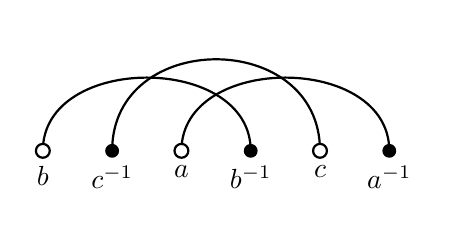
\begin{tikzpicture}[x=.88cm,y=.62cm,thick]
\foreach \i/\j/\h in {1/4/2,2/5/2.5,3/6/2}
 \draw (\i,0) .. controls (\i,\h) and (\j,\h) .. (\j,0);
\foreach \i in {1,3,5}\draw[fill=white] (\i,0) circle (2.5pt);
\foreach \i in {2,4,6}\fill (\i,0) circle (2.5pt);
\foreach \i/\w in {1/b,2/c^{-1},3/a,4/b^{-1},5/c,6/a^{-1}}
 \node[below] at (\i,-.1){$\w$};
\end{tikzpicture}
\end{center}

Indeed, with the labels shown, the relation reads $b\,c^{-1}a\,b^{-1}c\,a^{-1}=x_0y_0^{-1}x_0^{-1}y_0=1$.

Conversely, in the group from the statement, we can cancel as before the 2 letters coming from an innermost string labeled $b$ or $c$, because the letters between them come from strings which cross it. Thus all the relations coming from $I_D$ hold. Finally, for $k\in D$ we can send $x_0,y_k$ to the standard generators of $F_2$, and all the other elements $x_j,y_j$ to $1$. Observe that the elements $x_0,y_k$ are distinct generators even at $k=0$.
\end{proof}

The same method applies to any $N$. The dual of the diagonal torus of $U_N^D$ is generated by $a$ and by $N-1$ families of translates, which commute at the distances outside $D$, and are free at the distances inside $D$. In what follows we will only need Theorem~\ref{three-torus}, which proves Theorem~\ref{intro-torus}. Observe also that the first positive integer $m\in D$, and the number $t\in\{1,2\}$, which will play a key role in what follows, can be read on the torus:
\[
 m=\min\big\{k\geq1\,\big|\,x_0x_k\neq x_kx_0\big\},\qquad t=1\iff x_0y_0\neq y_0x_0.
\]

We will see in Section~\ref{examples} that the product $tm$ of these 2 numbers is the largest dimension where the diagonal entries of the reflection partner are free.

\section{Reflections on the integer line}\label{reflection}

We have seen that $D$ can be read on 3 diagonal coordinates of $U_N^D$, via certain commutation relations. We construct now the reflection partner, by using the opposite commutation relations. Let us begin with the following definition:

\begin{defn}\label{w-group}
Let $D\subset\mathbb N_0$ be a nonempty additive semigroup. When $0\in D$ we set
\[
 W_D=\Big\langle s_i\ (i\in\mathbb Z)\ \Big|\ s_i^2=1,\ s_is_j=s_js_i\ \text{when }i\neq j,\ |i-j|\in D\Big\rangle.
\]
When $0\notin D$ we use $2$ generators $s_i,s_i'$ of order $2$ at each integer $i$, with the relations stating that a generator at $i$ commutes with a generator at $j$ when $i\neq j$ and $|i-j|\in D$. In both cases, when $1\in D$, we only keep the generators at $i=0$. The generators of $W_D$ are called standard reflections, and the integer $i$ is called height of $s_i,s_i'$.
\end{defn}

In other words, 2 distinct standard reflections commute when their heights are different, at a distance belonging to $D$, and are free otherwise. In particular, when $0\notin D$, the 2 standard reflections $s_i,s_i'$ at a given height are free. As before, we denote by $t\in\{1,2\}$ the number of standard reflections at each height. Here are some examples:

(1) For $D=\mathbb N_0$ we have $W_D=\mathbb Z_2$, generated by $s_0$. Observe that without the convention regarding the case $1\in D$ we would obtain commuting reflections $s_i$, which, as we will soon see, lead to the same reflection partner.

(2) For $D=\{1,2,3,\ldots\}$ we have $W_D=\mathbb Z_2*\mathbb Z_2$, generated by $s_0,s_0'$. Here the convention regarding $1\in D$ is important. It is designed in order to have $H_N^*$ as partner of $U_N^\times$.

(3) For $D=\{0\}$ there are no commutation relations, and $W_D=\mathbb Z_2^{*\infty}$ is a free product.

(4) For $D_*=\{0,2,3,\ldots\}$ we have $s_is_j=s_js_i$ when $|i-j|\geq2$, and $s_i,s_{i+1}$ are free.

(5) For $D=d\mathbb N_0$ with $d\geq2$, the reflections $s_i,s_j$ commute when $i,j$ are congruent modulo $d$, and are free otherwise. Thus, $W_D$ is a free product of $d$ infinite sums of copies of $\mathbb Z_2$.

We will often use the following elementary fact. Given a set $R$ of standard reflections of $W_D$, we can send the standard reflections which are not in $R$ to $1$. This preserves the relations of $W_D$, and so the subgroup $\langle R\rangle\subset W_D$ is the group generated by the elements of $R$, with their squares being $1$, and with the commutation relations between them as only relations. See Lemma~\ref{retraction} below.

Consider now the free product $P_N=\mathbb Z_2^{*N}$, with standard generators $g_1,\ldots,g_N$. Any choice $r=(r_1,\ldots,r_N)$ of standard reflections of $W_D$, with repetitions allowed, produces a group morphism $\pi_r:P_N\to W_D$, given by $g_i\to r_i$. We also have a morphism $\varepsilon:P_N\to\mathbb Z_2^N$, mapping the generators $g_i$ to the standard generators of $\mathbb Z_2^N$, that we call commuting signs.

\begin{defn}\label{dprime}
We let $D'[N]$ be the quotient of $P_N=\langle g_1,\ldots,g_N\rangle$ by the relations which hold for commuting signs, and for any choice of standard reflections of $W_D$:
\[
 D'[N]=P_N\Big/\Big(\ker\varepsilon\cap\bigcap_r\ker\pi_r\Big).
\]
We denote by $D'$ the group obtained in the same way, with generators $g_1,g_2,g_3,\ldots$
\end{defn}

Equivalently, $D'[N]$ is the subgroup of the product of $\mathbb Z_2^N$ with copies of $W_D$, one copy for each choice $r$, generated by the following elements:
\[
 g_i=\big(\varepsilon(g_i),(r_i)_r\big)\in\mathbb Z_2^N\times\prod_rW_D.
\]

Observe that a relation between $g_1,\ldots,g_N$ holds in $D'$ precisely when it holds in $D'[N]$, because any choice of $N$ standard reflections extends to a choice of infinitely many. Thus $D'[N]$ is the subgroup of $D'$ generated by $g_1,\ldots,g_N$. Observe also that the condition regarding the commuting signs, which states that each generator appears an even number of times in our relation, is automatic when $W_D$ has at least 2 standard reflections $s\neq s'$. Indeed, we can choose $r_i=s$ and $r_j=s'$ for $j\neq i$, and then send $s'\to1$, as explained above. What is left is $s$ to the power the number of occurrences of $g_i$.

Let us recall now the construction of Raum and Weber. Consider a group $\Gamma$ generated by elements $g_1,g_2,g_3,\ldots$ of order 2, whose relations hold for commuting signs, and are preserved by any relabeling $g_i\to g_{\varphi(i)}$ of the generators, with $\varphi:\mathbb N\to\mathbb N$ being an arbitrary map. With $\Gamma_N=\langle g_1,\ldots,g_N\rangle$, it is shown in \cite{rw} that we have an easy quantum group $H_N^\Gamma$, with
\[
 C(H_N^\Gamma)=C^*(\Gamma_N)\otimes C(S_N),\qquad u_{ij}=g_i\otimes p_{ij}
\]
where $p_{ij}\in C(S_N)$ are the standard coordinates of the permutation group $S_N$, namely $p_{ij}(\sigma)=1$ when $\sigma(j)=i$, and $p_{ij}(\sigma)=0$ otherwise. The comultiplication is the one making $u$ a corepresentation. In the case where there are no relations at all, apart from $g_i^2=1$, the quantum group that we obtain is denoted $H_N^{[\infty]}$. All this applies to our situation, as follows:

\begin{prop}\label{partner-exists}
The group $D'$ satisfies the above conditions, and so produces an easy quantum group $H_N^{D'}$, that we call reflection partner of $U_N^D$. We have
\[
 H_N\subset H_N^{D'}\subset H_N^{[\infty]}\subset H_N^+
\]
and the diagonal torus of $H_N^{D'}$ is the group dual $\widehat{D'[N]}$.
\end{prop}

\begin{proof}
Let $w$ be a relation of $D'$, and consider a relabeling $g_i\to g_{\varphi(i)}$. In the relabeled word each generator still appears an even number of times. Also, evaluating the relabeled word at a choice $r$ of standard reflections is the same as evaluating $w$ at another choice, namely
\[
 r'=(r_{\varphi(1)},r_{\varphi(2)},r_{\varphi(3)},\ldots)
\]
so we obtain $1$. Thus the construction from \cite{rw} applies. The inclusions on the right are clear. The inclusion on the left comes from the fact that the commuting signs are a quotient of $D'[N]$. Finally, in order to compute the diagonal torus, we must set $g_i\otimes p_{ij}=0$ for $i\neq j$. By taking squares we obtain $p_{ij}=0$ for $i\neq j$, and so $p_{ii}=1$, and we are left with the algebra $C^*(D'[N])$.
\end{proof}

Here is now a more concrete description of the reflection partner, which is the one given in the Introduction. Given a choice $r=(r_1,\ldots,r_N)$ of standard reflections of $W_D$, the dual of the group $\langle r_1,\ldots,r_N\rangle$ is a closed subgroup of $H_N^+$, with fundamental representation $diag(r_1,\ldots,r_N)$. Observe that we have equal diagonal entries when $r_i=r_j$.

\begin{thm}\label{generation}
The reflection partner of $U_N^D$ is given by
\[
 H_N^{D'}=\Big\langle H_N,\ \widehat{\langle r_1,\ldots,r_N\rangle}\ \Big|\ r_1,\ldots,r_N\ \text{standard reflections of }W_D\Big\rangle
\]
as a closed subgroup of $H_N^+$. Moreover, finitely many choices of $r_1,\ldots,r_N$ suffice.
\end{thm}

\begin{proof}
Let $G$ be the quantum group on the right. We proceed in several steps.

(1) The group duals in the statement are subgroups of the diagonal torus of $H_N^{D'}$, because the groups $\langle r_1,\ldots,r_N\rangle$ are by definition quotients of $D'[N]$. Together with Proposition~\ref{partner-exists}, this gives $G\subset H_N^{D'}$.

(2) Conversely, $G$ contains the diagonal torus of $H_N^{D'}$. Indeed, let $\Lambda$ be the dual of the diagonal torus of $G$. By (1), and by the definition of $G$, we have quotient maps as follows, with $\mathbb Z_2^N$ coming from $H_N$, which are compatible with the standard generators:
\[
 D'[N]\to\Lambda\to\mathbb Z_2^N,\qquad D'[N]\to\Lambda\to\langle r_1,\ldots,r_N\rangle.
\]

But by definition of $D'[N]$, an element which is killed by all these composed maps is trivial. Thus the map on the left is injective, and so $\Lambda=D'[N]$.

(3) Thus $G\subset H_N^{D'}$ contains both the diagonal torus $\widehat{D'[N]}$ and the group $S_N\subset H_N$. Consider the comultiplication of $C(G)$, followed by the restriction to the diagonal torus on the left, and by the restriction to $S_N$ on the right. On the standard coordinates, we obtain
\[
 u_{ij}\to\sum_ku_{ik}\otimes u_{kj}\to\sum_k\delta_{ik}\,g_i\otimes p_{kj}=g_i\otimes p_{ij}.
\]

Thus our map, when composed with the quotient map $C(H_N^{D'})\to C(G)$, becomes injective on the $*$-algebra generated by the coordinates. We conclude that the quotient map is injective too, and so $G=H_N^{D'}$.

(4) Finally, as explained after Definition~\ref{w-group}, the group $\langle r_1,\ldots,r_N\rangle$, with its generators, only depends on which of the reflections $r_i$ coincide, and on which of them commute. Thus, there are finitely many groups involved.
\end{proof}

The situation is summarized by the following diagram:

\begin{figure}[H]\centering
\begin{tikzpicture}[x=1cm,y=1cm,>=stealth,inner sep=3pt,font=\small]
\node (whole) at (0,1.38) {$H_N^{D'}$};
\node (real) at (-3.0,0) {$H_N$};
\node (diag) at (3.0,0) {$\widehat{D'[N]}$};
\node (signs) at (0,-1.30) {$\mathbb Z_2^N$};
\draw[->] (signs)--(real);\draw[->] (signs)--(diag);
\draw[->] (real)--(whole);\draw[->] (diag)--(whole);
\node[anchor=east] at (-3.45,0) {signed permutations};
\node[anchor=west] at (3.82,0) {diagonal torus};
\end{tikzpicture}
\caption{The signed permutations and the diagonal torus generate the reflection partner. The diagonal torus is in turn generated by the duals of the groups $\langle r_1,\ldots,r_N\rangle$.}
\end{figure}

Let us work out the simplest examples. For $D=\mathbb N_0$ the only standard reflection is $s_0$, so the only choice is $r_i=s_0$ for any $i$, and the corresponding group dual is contained in $H_N$. Thus $H_N^{D'}=H_N$. The same happens for the group with commuting reflections $s_i$ mentioned after Definition~\ref{w-group}, because the duals of abelian groups generated by reflections, with diagonal fundamental representation, are contained in $H_N$. For $D=\{0\}$ we can choose distinct reflections $r_1,\ldots,r_N$, which are free. Thus $D'[N]=P_N$, and we obtain $H_N^{D'}=H_N^{[\infty]}$.

We can now prove that the correspondence reverses inclusions:

\begin{thm}\label{torus-partner}
For nonempty additive semigroups $D\subset E$ we have
\[
 U_N^D\subset U_N^E,\qquad H_N^{E'}\subset H_N^{D'}
\]
at any $N$, with all quantum groups being taken with their fundamental representations.
\end{thm}

\begin{proof}
The first inclusion is known from Theorem~\ref{mang-weber}. Regarding the second inclusion, we claim that any group $\langle r_1,\ldots,r_N\rangle$ coming from standard reflections of $W_E$ is a quotient of a group $\langle\tilde r_1,\ldots,\tilde r_N\rangle$ coming from standard reflections of $W_D$, via $\tilde r_i\to r_i$. By Theorem~\ref{generation}, this gives the result. In order to prove the claim, we lift the standard reflections of $W_E$, by keeping the heights. That is, we use the following lifts, with the second one being needed only when $0\notin E$:
\[
 s_i\to s_i,\qquad s_i'\to s_i'.
\]

Observe that $0\notin E$ implies $0\notin D$, so this is possible. Observe also that when $W_E$ has reflections at the height $0$ only, the same heights exist in $W_D$. Now if 2 of our lifts commute, they have different heights $i\neq j$ with $|i-j|\in D$, and so $|i-j|\in E$, and the original reflections commute as well. Since the commutation relations are the only relations between the lifts, apart from those stating that their squares are $1$, this proves our claim.
\end{proof}

As a conclusion, the correspondence $U_N^D\to H_N^{D'}$ is now constructed, and reverses inclusions. Observe also that, according to the formulae at the end of Section~\ref{tori}, the group $W_D$ and so the reflection partner can be constructed directly from the diagonal torus of $U_3^D$.

\section{Detecting the diagonal subgroups}\label{detection}

Suppose that someone gives us the reflection partners $H_N^{D'}$, with their fundamental representations. Can we recover $D$? In this section and in the next one we show that this is indeed possible. The idea will be that of looking at the group duals inside $H_N^{D'}$, having a diagonal fundamental representation.

It is convenient to record the relations between reflections by a graph, and since freeness will be more important for us than commutation, we will join 2 reflections when they are free. To be more precise, to any finite graph $F$ having vertices $1,\ldots,n$ we associate the group
\[
 W(F)=\Big\langle s_1,\ldots,s_n\ \Big|\ s_i^2=1,\ s_is_j=s_js_i\text{ when }i\neq j\text{ are not joined}\Big\rangle.
\]

For instance the graph with 2 vertices and one edge gives $\mathbb Z_2*\mathbb Z_2$, the complete graph gives $P_n=\mathbb Z_2^{*n}$, and the path $1-2-3$ gives $(\mathbb Z_2\times\mathbb Z_2)*\mathbb Z_2$, with $s_1,s_3$ commuting. The same construction applies to infinite graphs. Our groups $W_D$ are of this type, coming from the graph $X_D$ having as vertices the standard reflections of $W_D$, with 2 of them being joined when they are free. Observe that $X_D$ is connected. Indeed, this is clear when $1\in D$, where $X_D$ is a point or an edge, and when $1\notin D$ the reflections at consecutive heights are joined.

We will use the following standard facts, concerning such groups:

\begin{lem}\label{retraction}
Let $F$ be a graph, finite or not, and let $F_0$ be a set of vertices of $F$, with the edges of $F$ between them.
\begin{enumerate}
\item The subgroup of $W(F)$ generated by the reflections $s_v$ with $v\in F_0$ is the group $W(F_0)$, and there is a retraction $W(F)\to W(F_0)$, mapping $s_v\to1$ for $v\notin F_0$.

\item The set of reflections $s_v$ appearing in a reduced word for an element $g\in W(F)$, called support of $g$, does not depend on the reduced word.

\item If $s_v$ is not in the support of $g$, and $v$ is joined to some vertex in the support of $g$, then the support of $s_vgs_v$ is the support of $g$, together with $s_v$.
\end{enumerate}
\end{lem}

\begin{proof}
The map $s_v\to s_v$ for $v\in F_0$, and $s_v\to1$ otherwise, preserves the relations of $W(F)$, so it defines a morphism $W(F)\to W(F_0)$. Together with the obvious morphism in the other sense, we have a composition as follows, which is the identity of $W(F_0)$:
\[
 W(F_0)\to W(F)\to W(F_0).
\]

Thus the map on the left is injective, and this proves (1). The assertion (2) is a basic property of graph products of groups \cite{green}. Indeed, any 2 reduced words for the same element are related by exchanging adjacent commuting letters. As for (3), this follows from the same normal form result, because the 2 copies of $s_v$ in the word $s_vgs_v$ cannot be moved through $g$ in order to cancel.
\end{proof}

Given a finite graph $F$ as above, the dual of $W(F)$ is a closed subgroup of $H_n^+$, with fundamental representation $diag(s_1,\ldots,s_n)$. We want to know whether this diagonal group dual is contained in $H_n^{D'}$. Equivalently, we want to know whether $g_i\to s_i$ defines a group morphism $D'[n]\to W(F)$. We say that $F$ fits in $X_D$ when we can find distinct standard reflections $r_1,\ldots,r_n$ of $W_D$ such that $r_i,r_j$ are free whenever $i,j$ are joined in $F$. Thus, the vertices of $F$ must go to distinct vertices of $X_D$, with all the edges being preserved, and with extra edges in $X_D$ being allowed.

\begin{figure}[H]\centering
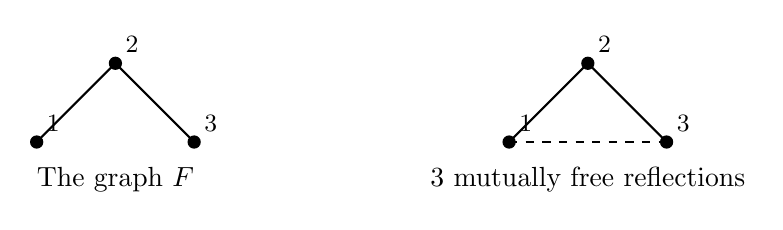
\begin{tikzpicture}[x=1cm,y=1cm,thick]
\foreach \d in {0,6}{
\draw (\d,0)--(\d+1,1)--(\d+2,0);
\foreach \x/\y/\i in {0/0/1,1/1/2,2/0/3}{\fill (\d+\x,\y) circle (2.4pt);
\node[above right,font=\small] at (\d+\x,\y){$\i$};}}
\draw[dashed] (6,0)--(8,0);
\node at (1,-.48){The graph $F$};\node at (7,-.48){3 mutually free reflections};
\end{tikzpicture}
\caption{The path with 3 vertices fits in a triangle. Imposing the commutation of the endpoint reflections gives a quotient map $\mathbb Z_2^{*3}\to(\mathbb Z_2\times\mathbb Z_2)*\mathbb Z_2$.}
\label{path-triangle}
\end{figure}

The answer to our question will be that $\widehat{W(F)}\subset H_n^{D'}$ happens precisely when $F$ fits in $X_D$, provided that $F$ is connected. One implication is elementary, as illustrated above. For the other one, we need a technical result, as follows:

\begin{lem}\label{centralizer}
Let $F$ be a finite connected graph, with at least $3$ vertices. Then any $2$ nontrivial normal subgroups of $W(F)$ contain elements which do not commute.
\end{lem}

\begin{proof}
We use an action of $W=W(F)$ on a tree, the idea being as follows:

(1) Choose a vertex $v$ having at least 2 neighbors. Let $A\subset W$ be the subgroup generated by all the reflections except for $s_v$, let $C\subset A$ be the subgroup generated by the reflections which commute with $s_v$, and set $B=C\times\langle s_v\rangle$. By Lemma~\ref{retraction} these subgroups are given by the corresponding parts of the presentation of $W$, and so we have an amalgamated free product decomposition, as follows:
\[
 W=A*_CB.
\]

Consider the tree $T$ associated to this decomposition \cite{trees}. Its vertices are the cosets $gA$ and $gB$, and its edges are the cosets $gC$, with $gC$ joining $gA$ and $gB$. The group $W$ acts on $T$, by left multiplication. Each vertex $gB$ has 2 neighbors, and each vertex $gA$ has $[A:C]\geq4$ neighbors. Indeed, with $a,b$ being 2 neighbors of $v$, the retraction of $A$ onto $\langle s_a,s_b\rangle$ kills $C$, and the group $\langle s_a,s_b\rangle$ has at least 4 elements. Thus, the tree looks as follows:

\begin{figure}[H]\centering
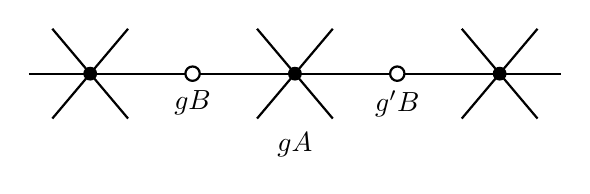
\begin{tikzpicture}[x=1.3cm,y=.6cm,thick]
\draw (-.6,0)--(4.6,0);
\foreach \x in {0,2,4} {
 \draw (\x-.37,.95)--(\x,0)--(\x+.37,-.95);
 \draw (\x+.37,.95)--(\x,0)--(\x-.37,-.95);
 \fill (\x,0) circle (2.5pt);}
\foreach \x in {1,3} \draw[fill=white] (\x,0) circle (2.6pt);
\node[below] at (1,-.15){$gB$};\node[below] at (3,-.15){$g'B$};
\node at (2,-1.5){$gA$};
\end{tikzpicture}
\caption{A part of the tree $T$. The white vertices are the cosets of $B$, and have 2 neighbors. The black vertices are the cosets of $A$, and have at least 4 neighbors.}
\end{figure}

(2) The action has no fixed vertex, because $A,B\neq W$, and all the edges are in the same orbit. Thus, the only nonempty invariant subtree is $T$ itself. Also, the action fixes no end of $T$. Indeed, the stabilizer of a vertex acts transitively on the edges at that vertex, whereas a fixed end would distinguish one of these edges, the one pointing towards it.

(3) The action is faithful. Indeed, its kernel $K$ is a normal subgroup, contained in the stabilizer $C$ of an edge. Assume that we have $g\in K$ with $g\neq1$. Since $F$ is connected, by using Lemma~\ref{retraction} (3) several times we can conjugate $g$ to an element whose support consists of all the reflections. But such an element cannot belong to $C$.

(4) We claim that any normal subgroup $M\neq\{1\}$ contains a translation of $T$. Recall from \cite{trees} that each $g\in W$ either fixes a vertex, or is a translation along a line, called its axis. Assume that all the elements of $M$ fix vertices. Then by \cite{trees} any finitely generated subgroup of $M$ fixes a vertex. Write $M$ as an increasing union of finitely generated subgroups $M_n$, and let $T_n\subset T$ be the subtree of vertices fixed by $M_n$. We have then
\[
 M_1\subset M_2\subset M_3\subset\ldots,\qquad T_1\supset T_2\supset T_3\supset\ldots
\]

If the subtrees $T_n$ have a common vertex then the set of vertices fixed by $M$ is a nonempty subtree, which is invariant, since $M$ is normal. By (2) this subtree is $T$, and so by (3) we have $M=\{1\}$, contradiction. 

If the subtrees $T_n$ have no common vertex, fix a vertex $p$, and let $p_n$ be the vertex of $T_n$ which is closest to $p$. Since $T_{n+1}\subset T_n$, the paths from $p$ to $p_n$ are increasing, and their union is an infinite ray, defining an end $\omega$ of $T$:
\[
 p\to p_1\to p_2\to p_3\to\ldots\to\omega.
\]
 Each $M_n$ fixes the vertices $p_k$ with $k\geq n$, so $M$ fixes $\omega$. Moreover, $\omega$ is the only end fixed by $M$. Indeed, an element which fixes 2 ends and a vertex must fix all the vertices of the line joining these ends, so $M$ would fix vertices. Thus, since $M$ is normal, $\omega$ is fixed by $W$, which contradicts (2).

(5) Assume now that $M,M'\neq\{1\}$ are normal subgroups commuting with each other, and choose translations $h\in M$ and $k\in M'$. Since $k$ commutes with $h$, it preserves the axis of $h$, and so this is the axis of $k$ too. The same holds for any conjugate $ghg^{-1}\in M$, and so we have, for any $g\in W$:
\[
 g\cdot axis(h)=axis(ghg^{-1})=axis(k)=axis(h).
\]

Thus the axis of $h$ is invariant under $W$, which contradicts (2), because by (1) the tree $T$ is not a line.
\end{proof}

We can now answer the question raised above, as follows:

\begin{thm}\label{test}
Let $F$ be a finite connected graph, with vertices $1,\ldots,n$. We have
\[
 \widehat{W(F)}\subset H_n^{D'}
\]
with fundamental representation $diag(s_1,\ldots,s_n)$, if and only if $F$ fits in $X_D$.
\end{thm}

\begin{proof}
Assume first that $F$ fits in $X_D$, via standard reflections $r_1,\ldots,r_n$. If $r_i,r_j$ commute then $i,j$ are not joined in $F$, so $s_i,s_j$ commute too. By Lemma~\ref{retraction} we obtain a quotient map $\langle r_1,\ldots,r_n\rangle\to W(F)$, given by $r_i\to s_i$, and so $\widehat{W(F)}\subset H_n^{D'}$, by Theorem~\ref{generation}.

Conversely, assume that $F$ does not fit in $X_D$. We must find a word $w$ in the generators $g_1,\ldots,g_n$ of $P_n$ which is a relation of $D'[n]$, but which survives in $W(F)$, via $g_i\to s_i$.

At $n\leq2$ this is clear. Indeed, at $n=1$ any graph fits. At $n=2$ the graph $F$ is an edge, with $W(F)=\mathbb Z_2*\mathbb Z_2$, and if it does not fit then any 2 standard reflections of $W_D$ coincide or commute, so $w=(g_1g_2)^2$ is a relation of $D'[2]$, surviving in $W(F)$.

At $n\geq3$, consider the finite list consisting of the following words:
\[
 g_ig_j\ \ (i<j),\qquad\quad(g_ig_j)^2\ \ (i,j\ \text{joined in}\ F).
\]

Any choice $r_1,\ldots,r_n$ of standard reflections kills one of these words. Indeed, if $r_i=r_j$ for some $i<j$ then $g_ig_j$ is killed. If the reflections $r_i$ are distinct then, since $F$ does not fit, we can find $i,j$ joined in $F$ with $r_i,r_j$ commuting, and $(g_ig_j)^2$ is killed. On the other hand, all the words in our list survive in $W(F)$, because distinct generators are distinct there, and because the endpoints of an edge are free.

Let now $A_1,\ldots,A_l\subset P_n$ be the normal subgroups generated by the words in our list, and consider the following iterated commutator subgroup:
\[
 M=\big[\ldots\big[[A_1,A_2],A_3\big],\ldots,A_l\big].
\]

This is contained in each $A_i$, so the elements of $M$ are killed by any choice of standard reflections, and since $l\geq2$ they hold as well for commuting signs. Thus, the elements of $M$ are relations of $D'[n]$. On the other hand, the images of $A_1,\ldots,A_l$ in $W(F)$ are nontrivial normal subgroups, so by using Lemma~\ref{centralizer} several times, the image of $M$ in $W(F)$ is nontrivial. Thus, we can find $w\in M$ as desired.
\end{proof}

As a consequence, the reflection partners, taken in all dimensions, know which finite connected graphs fit in $X_D$. Let us denote by $T(X_D)$ the set of such graphs, taken up to isomorphism. The complete result here is as follows:

\begin{thm}\label{order}
For nonempty additive semigroups $D,E\subset\mathbb N_0$, we have $H_N^{D'}\subset H_N^{E'}$ for any $N$ if and only if $T(X_D)\subset T(X_E)$. In particular, we have
\[
 H^{D'}=H^{E'}\iff T(X_D)=T(X_E)
\]
with the equality on the left being in all dimensions.
\end{thm}

\begin{proof}
If $H_n^{D'}\subset H_n^{E'}$ for any $n$ then any diagonal group dual inside $H_n^{D'}$ is inside $H_n^{E'}$, and Theorem~\ref{test} gives $T(X_D)\subset T(X_E)$. Conversely, assume $T(X_D)\subset T(X_E)$. We must prove that any relation of $E'[n]$ is a relation of $D'[n]$. So, let $w$ be a word in $g_1,\ldots,g_n$ which is not a relation of $D'[n]$. If $w$ fails for commuting signs, it is not a relation of $E'[n]$ either. Otherwise we can find standard reflections $r_1,\ldots,r_n$ of $W_D$ such that
\[
 w(r_1,\ldots,r_n)\neq1.
\]

Since $X_D$ is connected, we can find a finite set $R$ of standard reflections, containing $r_1,\ldots,r_n$, and forming a connected graph. By our assumption this graph fits in $X_E$, so we can find distinct standard reflections $\rho(q)$ of $W_E$, with $q\in R$, such that $\rho(q),\rho(q')$ are free whenever $q,q'$ are free. As in the proof of Theorem~\ref{test}, we obtain a quotient map $\langle\rho(R)\rangle\to\langle R\rangle$ given by $\rho(q)\to q$, and this quotient map acts as follows:
\[
 w(\rho(r_1),\ldots,\rho(r_n))\to w(r_1,\ldots,r_n)\neq1.
\]

Thus $w$ is not a relation of $E'[n]$, as desired.
\end{proof}

\section{Reconstruction of the semigroup}\label{recover}

We know from Theorem~\ref{order} that the reflection partners, taken in all dimensions, determine the finite connected graphs which fit in $X_D$. However, in these graphs the reflections no longer carry their heights. In this section we recover $D$ from these graphs.

Let us first have a closer look at the graph $X_D$. Assume $D\neq\{0\}$, let $d$ be the greatest common divisor of the positive elements of $D$, and write
\[
 D\cup\{0\}=dS.
\]

Then $S$ is an additive semigroup containing $0$, whose positive elements have greatest common divisor $1$. Such semigroups are called numerical semigroups, and it is well-known that the complement $B=\mathbb N_0-S$, whose elements are called gaps, is finite. See \cite{rgs}. Indeed, if $a\in S$ is positive, the residues modulo $a$ of the elements of $S$ form a subgroup of $\mathbb Z_a$, which must be $\mathbb Z_a$ itself. By choosing an element of $S$ in each residue class, and adding multiples of $a$, we see that $S$ contains all the integers which are big enough. As before, we denote by $t\in\{1,2\}$ the number of reflections at each height. Observe that we have $1\in D$ precisely when $d=1$ and $B=\emptyset$.

Let us call line the set of standard reflections of $W_D$ having heights in a given residue class modulo $d$. On each of the $d$ lines, we number the heights $r+dj$ by the integer $j$. Then:

(1) Reflections on different lines are always free, because the difference between their heights is not a multiple of $d$, and so is not in $D$.

(2) Reflections on the same line, at the heights numbered $j\neq j'$, are free precisely when $|j-j'|\in B$. At $t=2$, the 2 reflections at each height are free as well.

In terms of graphs, let us agree, as in Section~\ref{detection}, that a finite graph $F$ fits in a graph $Y$ when the vertices of $F$ can be sent to distinct vertices of $Y$, with any 2 vertices which are joined being sent to vertices which are joined. Let us also denote by $Y_B^t$ the graph having vertices $(j,e)$ with $j\in\mathbb Z$ and $e\in\{1,\ldots,t\}$, with $(j,e)$ and $(j',e')$ being joined when $|j-j'|\in B$, or when $j=j'$ and $e\neq e'$. Also, given a graph $Y$, we denote by $J_d(Y)$ the graph consisting of $d$ disjoint copies of $Y$, with any 2 vertices in different copies being joined. With these conventions, for $1\notin D$ we have
\[
 X_D=J_d(Y_B^t).
\]

As an illustration, for $2D_*=\{0,4,6,8,\ldots\}$ we have $d=2$ and $B=\{1\}$. The 2 lines consist of the even and odd integers, and on each line the neighbors are free:

\begin{figure}[H]\centering
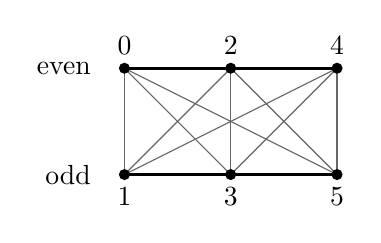
\begin{tikzpicture}[x=1.35cm,y=1.35cm,thick]
\foreach \x in {0,1,2}\foreach \z in {0,1,2}\draw[thin,black!60] (\x,1)--(\z,0);
\draw[very thick] (0,1)--(2,1) (0,0)--(2,0);
\foreach \x in {0,1,2}{\fill (\x,1) circle (2pt) (\x,0) circle (2pt);
\node[above] at (\x,1.03){$\the\numexpr 2*\x\relax$};
\node[below] at (\x,-.03){$\the\numexpr 2*\x+1\relax$};}
\node[left] at (-.22,1){even};\node[left] at (-.22,0){odd};
\end{tikzpicture}
\caption{A part of the graph $X_D$ for $D=2D_*$. Each line is a path, and any reflection on the even line is free from any reflection on the odd line.}
\label{residue-lines}
\end{figure}

In group-theoretic terms, the above description shows that $W_D$ is a free product of $d$ copies of the group associated to a line. We first recover the number of lines:

\begin{lem}\label{lines}
Let $Y$ be an infinite graph, whose vertices have at most $\Delta<\infty$ neighbors.
\begin{enumerate}
\item The graph consisting of $r$ sets of $u$ vertices, with $2$ vertices being joined when they belong to different sets, fits in $J_d(Y)$ for any $u$ precisely when $r\leq d$.

\item Assume $d\geq2$. A finite graph $F$ fits in $Y$ precisely when $J_d(F_u)$ fits in $J_d(Y)$ for any $u$, where $F_u$ is the graph $F$, together with $u$ isolated vertices.
\end{enumerate}
\end{lem}

\begin{proof}
(1) When $r\leq d$ we can put each set on its own line. Conversely, assume $r>d$ and $u>d\Delta$. Each of the $r$ sets has more than $\Delta$ vertices on some line, and since $r>d$, we can find 2 sets and a line containing more than $\Delta$ vertices of each of them. But then a vertex of the first set has more than $\Delta$ neighbors on its line, which is impossible.

(2) If $F$ fits in $Y$ then so does $F_u$, because $Y$ is infinite, and only the edges of $F_u$ must be preserved. Thus $J_d(F_u)$ fits in $J_d(Y)$. Conversely, assume that $J_d(F_u)$ fits in $J_d(Y)$, with $u>d\Delta$. Each of the $d$ copies of $F_u$ has more than $\Delta$ of its isolated vertices on some line. As in the proof of (1), these $d$ lines are distinct, and a vertex of another copy cannot be on such a line, because it would have more than $\Delta$ neighbors there. Thus each copy of $F_u$ is on a single line, and so $F$ fits in $Y$.
\end{proof}

\begin{figure}[H]\centering
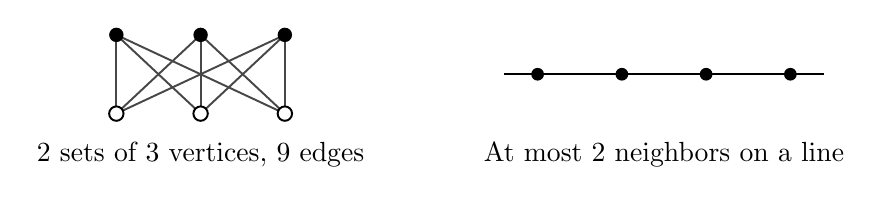
\begin{tikzpicture}[x=1.07cm,y=1cm,line width=.7pt]
\foreach \i in {0,1,2}\foreach \j in {0,1,2}\draw[black!72] (\i,1)--(\j,0);
\foreach \i in {0,1,2}{\fill (\i,1) circle (2.6pt);
 \draw[fill=white] (\i,0) circle (2.6pt);}
\begin{scope}[shift={(5,.5)}]
 \draw (-.4,0)--(3.4,0);
 \foreach \i in {0,1,2,3}\fill (\i,0) circle(2.3pt);
\end{scope}
\node at (1,-.52){2 sets of 3 vertices, 9 edges};
\node at (6.5,-.52){At most 2 neighbors on a line};
\end{tikzpicture}
\caption{The idea of the proof, with $r=2$ and $u=3$. The graph on the left fits in 2 different lines, but not in a single line which is a path.}
\label{line-count}
\end{figure}

Next, we must reconstruct a line. Given a graph $Y$ and a vertex $v$, we denote by $Y(v,R)$ the ball of radius $R$ around $v$, that is, the graph formed by the vertices which can be reached from $v$ by a path having at most $R$ edges, with the edges of $Y$ between them.

\begin{lem}\label{balls}
Let $Y,Y'$ be graphs in which each vertex has exactly $q<\infty$ neighbors, and assume that $Y(v,R+1)$ fits in $Y'$, via a map $\varphi$. Then $\varphi$ restricts to an isomorphism
\[
 Y(v,R)\simeq Y'(\varphi(v),R)
\]
which maps the neighbors of any vertex $u$ onto the neighbors of $\varphi(u)$.
\end{lem}

\begin{proof}
Let $u$ be a vertex of $Y(v,R)$. Its $q$ neighbors are in $Y(v,R+1)$, and are mapped by $\varphi$ to $q$ distinct neighbors of $\varphi(u)$, which are therefore all the neighbors of $\varphi(u)$. Thus, with $N(u)$ standing for the set of neighbors of $u$, we have
\[
 \varphi(N(u))=N(\varphi(u))
\]
which proves the last assertion. Now since paths are mapped to paths, the image of $Y(v,r)$ is contained in $Y'(\varphi(v),r)$, for any $r\leq R$, and by induction on $r$ we have equality, because a vertex at distance $r$ from $\varphi(v)$ is a neighbor of a vertex at distance $r-1$. Finally, if $\varphi(u),\varphi(u')$ are joined, with $u,u'$ in $Y(v,R)$, then $\varphi(u')$ is among the neighbors of $\varphi(u)$, which are the images of the neighbors of $u$. Thus $u,u'$ are joined.
\end{proof}

We must now put numbers back on the vertices of a line. For a finite set $A$ of positive integers, let $Y_A=Y_A^1$ be the graph on $\mathbb Z$ having $i,j$ joined when $|i-j|\in A$. We call steps the elements of $A$.

\begin{figure}[H]\centering
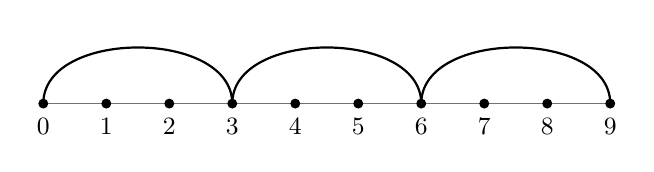
\begin{tikzpicture}[x=.8cm,y=1cm,line cap=round]
\draw[black!55] (0,0)--(9,0);
\foreach \i in {0,...,9}{\fill (\i,0) circle(1.8pt);\node[below,font=\small] at (\i,-.06){$\i$};}
\foreach \i in {0,3,6}\draw[thick] (\i,0) .. controls +(0,.95) and +(0,.95) .. (\i+3,0);
\end{tikzpicture}
\caption{The graph $Y_A$ with $A=\{1,3\}$. We show the steps of length $1$, and the 3 steps of length $3$ forming the unique shortest path from $0$ to $9$.}
\label{long-steps}
\end{figure}

The idea will be that the largest step can be recognized, as in the above picture, and then removed. To be more precise, we have the following result:

\begin{lem}\label{steps}
Let $A,A'\subset\{1,\ldots,g\}$ be sets of integers, both containing $1$, and both having $\gamma$ elements. If there is an isomorphism between the balls of radius $\gamma g$ around $0$ of the graphs $Y_A,Y_{A'}$, which maps $0\to0$, then $A=A'$.
\end{lem}

\begin{proof}
We first recognize the largest step $a=\max A$. We claim that for $w\in\mathbb Z$, the vertices which are at distance $g$ from $w$, and are joined to $w$ by only one path of length $g$, are
\[
 w+ga,\qquad w-ga.
\]

Indeed, in $g$ steps we can move by at most $ga$, with equality when all the steps are $a$, in the same direction. Conversely, consider a path of length $g$ between vertices at distance $g$, which is unique. By permuting its steps we obtain again a path of length $g$, with the same endpoints. Thus all the steps are equal, to a number $\pm c$ with $c\in A$. But if $c<a$ then, since $g\geq a$, we can replace $a$ steps of length $c$ by $c$ steps of length $a$, and obtain a path which is shorter, having length
\[
 g-a+c<g.
\]

Thus $c=a$, and our claim is proved.

Now let $\varphi$ be an isomorphism between the balls of radius $\rho$ around $0$ of $Y_A,Y_{A'}$, with $\varphi(0)=0$. Then $\varphi$ preserves the distance to $0$. If $w$ is at distance at most $\rho-g$ from $0$, the paths of length at most $g$ starting at $w$ stay inside the ball, and the same holds for $\varphi(w)$. Thus $\varphi$ maps the paths of length $g$ starting at $w$ to the paths of length $g$ starting at $\varphi(w)$, and distances from $w$ which are at most $g$ are preserved. By the above claim, with $a'=\max A'$, and since the unique paths in question must correspond to each other, we conclude that
\[
 \varphi(\{w+a,w-a\})=\{\varphi(w)+a',\varphi(w)-a'\}
\]
for any such $w$. In other words, $\varphi$ maps steps of length $a$ to steps of length $a'$.

Let us remove now the largest steps. Consider the sets $A_1=A-\{a\}$ and $A_1'=A'-\{a'\}$, and the corresponding graphs. A path from $0$ having at most $\rho-g$ steps in $Y_{A_1}$ is also a path in $Y_A$, and by the above its steps are mapped to steps of $Y_{A_1'}$. The same holds for $\varphi^{-1}$. Thus $\varphi$ restricts to an isomorphism between the balls of radius $\rho-g$ around $0$ of $Y_{A_1},Y_{A_1'}$.

Starting with $\rho=\gamma g$, we can repeat this procedure, with the radius decreasing as follows:
\[
 \gamma g\to(\gamma-1)g\to\ldots\to2g\to g.
\]

With $a_1>\ldots>a_\gamma=1$ and $a_1'>\ldots>a_\gamma'=1$ being the elements of $A,A'$, we obtain $\varphi(a_i)=\pm a_i'$ for any $i$, and after $\gamma-1$ removals we are left with an isomorphism between the balls of radius $g$ around $0$ of the graph $Y_{\{1\}}$, which is a path. Thus $\varphi(j)=ej$ for any $|j|\leq g$, for a certain sign $e=\pm1$. In particular $\varphi(a_i)=ea_i$, and by comparing with $\varphi(a_i)=\pm a_i'$ we obtain $a_i=a_i'$ for any $i$.
\end{proof}

Results of this type, for the full graphs instead of balls, are known in a more general setting, see \cite{morris}. We can now prove our main result, as follows:

\begin{thm}\label{main}
The correspondence $U^D\to H^{D'}$ is one-to-one, with $D$ ranging over the nonempty additive semigroups of $\mathbb N_0$, and with the quantum groups being compared in all dimensions. It reverses inclusions, and its image consists of $H^{[\infty]}$, and of exactly one quantum reflection group for each triple $(d,B,t)$ consisting of an integer $d\geq1$, of the set of gaps $B$ of a numerical semigroup, and of a number $t\in\{1,2\}$.
\end{thm}

\begin{proof}
The reversing of the inclusions was proved in Theorem~\ref{torus-partner}, and the description of the image follows from the above discussion, because the triple $(d,B,t)$ corresponds to the semigroup $D=d(\mathbb N_0-B)$, with $0$ removed when $t=2$. It remains to prove the injectivity. By Theorem~\ref{order}, we must prove that the set $T(X_D)$ of finite connected graphs fitting in $X_D$ determines $D$.

(1) We have $D=\{0\}$ precisely when all the finite complete graphs fit in $X_D$. Indeed, for $D=\{0\}$ all the standard reflections are free. Otherwise, let $m\in D$ be positive. Given standard reflections which are pairwise free, their heights must be distinct modulo $m$, up to the fact that at $t=2$ we can have $2$ reflections at each height. Thus, the number of such reflections is at most $tm$.

(2) We have $1\in D$ precisely when $X_D$ is finite. In this case $X_D$ is a point when $D=\mathbb N_0$, and an edge when $D=\{1,2,3,\ldots\}$, and $T(X_D)$ distinguishes these cases from each other, and from all the other cases, where arbitrarily large connected graphs fit in $X_D$.

(3) In the remaining cases we have $X_D=J_d(Y)$ with $Y=Y_B^t$, and $(d,B)\neq(1,\emptyset)$. The number of neighbors of each vertex of $Y$ is
\[
 q=t(2|B|+1)-1.
\]

By Lemma~\ref{lines} (1), applied with $r\geq2$, where the graphs involved are connected, $T(X_D)$ determines $d$. At $d=1$ we have $Y=X_D$. At $d\geq2$, by Lemma~\ref{lines} (2), where the graphs $J_d(F_u)$ are connected, $T(X_D)$ determines the set $T(Y)$ of finite connected graphs fitting in $Y$. The largest graph in $T(Y)$ consisting of a vertex joined to several other vertices gives $q$. Now $q$ is even at $t=1$, and odd at $t=2$. Thus we know $t$, and then $|B|$.

(4) If $|B|=0$ we are done. Otherwise $1\in B$, because an additive semigroup containing $1$ contains all the positive integers. Thus $Y$ is connected. Assume now that we have a second parameter, leading to a graph $Y'=Y_{B'}^t$ with $T(Y)=T(Y')$ and $|B|=|B'|=\gamma$. Let $g$ be the largest element of $B\cup B'$, let $v=(0,1)$, and set $R=\gamma g$. The ball $Y(v,R+1)$ is connected, so it fits in $Y'$, and since $Y'$ has enough symmetries, we can assume that the corresponding map $\varphi$ satisfies $\varphi(v)=v$. Lemma~\ref{balls} applies, and gives an isomorphism between the balls of radius $R$ around $v$. At $t=1$ we obtain $B=B'$, by Lemma~\ref{steps}.

(5) At $t=2$ we must first identify the 2 reflections at each height. Consider the closed neighborhood of a vertex, consisting of the vertex and of its neighbors. In $Y$ the vertices $(j,1),(j,2)$ have the same closed neighborhood, formed by the vertices having heights in the following set:
\[
 j+(\{0\}\cup B\cup-B).
\]

Since a finite set of integers cannot be equal to a nonzero translate of itself, vertices at different heights have different closed neighborhoods. By Lemma~\ref{balls}, $\varphi$ maps closed neighborhoods to closed neighborhoods, for the vertices of the ball of radius $R$ around $v$. Thus $\varphi$ maps pairs of reflections having the same height to pairs of the same type, and so induces an isomorphism between the balls of radius $R=\gamma g$ around $0$ of the graphs $Y_B,Y_{B'}$. Lemma~\ref{steps} gives again $B=B'$.
\end{proof}

The above result proves Theorem~\ref{intro-image}. Observe that it also explains why $D=\emptyset$ must be excluded. Indeed, at $D=\emptyset$ we would have 2 free reflections at each height, with all the reflections being free, exactly as for $D=\{0\}$. However, by Proposition~\ref{order-unitary} the unitary quantum groups $U^\emptyset$ and $U^{\{0\}}$ are different.

\section{Dimensions and half-liberations}\label{examples}

We have seen that the reflection partners, taken in all dimensions, determine $D$. What can we see in a single dimension? Let us begin with the simplest question, namely deciding when the diagonal entries of $H_N^{D'}$ are free, as for $H_N^{[\infty]}$. The answer is as follows:

\begin{thm}\label{dimension}
Let $D\neq\{0\}$, let $m$ be the smallest positive element of $D$, and let $t\in\{1,2\}$ be the number of standard reflections at each height. We have then
\[
 H_N^{D'}=H_N^{[\infty]}\iff D'[N]=P_N\iff N\leq tm
\]
with the equality in the middle being as groups with generators. For $D=\{0\}$ we have $H_N^{D'}=H_N^{[\infty]}$, in any dimension.
\end{thm}

\begin{proof}
The first equivalence is clear, because the quantum groups in question are determined by the corresponding groups, with their generators. Regarding now the second equivalence, by Theorem~\ref{test}, applied to the complete graph with $N$ vertices, we have $D'[N]=P_N$ precisely when we can find $N$ standard reflections of $W_D$ which are pairwise free. But we have seen in the proof of Theorem~\ref{main} that there are at most $tm$ such reflections. Conversely, consider the standard reflections at the following heights, which are $tm$ in number:
\[
 0,1,\ldots,m-1.
\]

These reflections are pairwise free, because the differences between these heights are smaller than $m$, and so are not in $D$. Thus we can find $N$ pairwise free standard reflections precisely when $N\leq tm$. Finally, the assertion regarding $D=\{0\}$ is already known.
\end{proof}

\begin{figure}[H]\centering
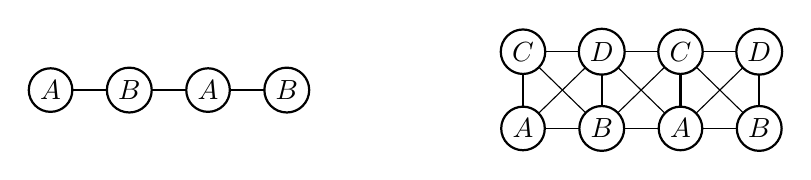
\begin{tikzpicture}[x=1cm,y=.84cm,thick]
\draw (0,0)--(3,0);
\foreach \x/\s in {0/A,1/B,2/A,3/B}{\node[circle,draw,fill=white,inner sep=2pt] at (\x,0){$\s$};}
\begin{scope}[shift={(6,-.58)}]
\foreach \x in {0,1,2}{\foreach \y in {0,1.16}\foreach \z in {0,1.16}\draw[thin] (\x,\y)--(\x+1,\z);}
\foreach \x in {0,1,2,3}\draw (\x,0)--(\x,1.16);
\foreach \x/\s/\t in {0/A/C,1/B/D,2/A/C,3/B/D}{
\node[circle,draw,fill=white,inner sep=2pt] at (\x,0){$\s$};
\node[circle,draw,fill=white,inner sep=2pt] at (\x,1.16){$\t$};}
\end{scope}
\end{tikzpicture}
\caption{The case $m=2$, for $D_*=\{0,2,3,\ldots\}$ on the left, and for $Q=\{2,3,4,\ldots\}$ on the right. Reflections with the same letter commute, so there are at most 2, respectively 4 pairwise free reflections.}
\label{path-colors}
\end{figure}

The above result proves Theorem~\ref{intro-embedding}. Observe that, in view of the formulae at the end of Section~\ref{tori}, the largest dimension where the diagonal of the reflection partner is free can be read on the diagonal torus of $U_3^D$. Indeed, $m$ is the first positive integer $k$ such that $x_0,x_k$ do not commute, and we have $t=2$ precisely when $x_0,y_0$ commute.

There is a useful way of thinking about all this. Consider the following relation on the integers, which is a partial order when $0\in D$, due to the fact that $D$ is an additive semigroup:
\[
 i\preceq j\iff j-i\in D.
\]

With this convention, 2 distinct standard reflections $s_i,s_j$ commute when $i,j$ are comparable, and are free when $i,j$ are incomparable. Thus, the sets of pairwise free reflections correspond to the antichains, and Theorem~\ref{dimension} tells us that the largest antichains have $m$ elements. Observe that the integers split into $m$ chains, namely the residue classes modulo $m$, in agreement with the Dilworth theorem \cite{dilworth}. We will come back to this order in Section~\ref{unitary-laws}.

As an illustration for Theorem~\ref{dimension}, consider the path $D_*=\{0,2,3,\ldots\}$. Here $tm=2$, so the first relation appears in dimension 3. With $a,b,c$ being the 3 diagonal generators, for any choice of standard reflections, at least one of the commutators $[a,b],[b,c],[c,a]$ is trivial. Thus
\[
 \big[\big[[a,b],[b,c]\big],[c,a]\big]=1
\]
is a relation, with $[x,y]=xyx^{-1}y^{-1}$. This is a relation between the standard generators, although the pair which commutes depends on the choice of the reflections. Let us check that the word on the left is nontrivial in $P_3$. With $p=[a,b]=abab$ and $q=[b,c]=bcbc$, the reduced word for $[p,q]$ begins with $a$ and ends with $cb$. Thus, the reduced word for $[p,q]\,caca$ begins with $a$, while in $caca\,[p,q]$ the initial $a$ of $[p,q]$ cancels, and the reduced word begins with $c$. Thus $[p,q]$ does not commute with $[c,a]=caca$. We will see in Section~\ref{reflection-laws} that the shortest relations for the path have length 30.

Let us discuss now some basic families of examples. There are 2 simple ways of enlarging a reflection partner, namely adding gaps on a single line, or adding lines:

\begin{prop}\label{series}
Let $D_m=\{0\}\cup\{m,m+1,\ldots\}$ and $E_d=d\mathbb N_0$. We have strict inclusions
\[
 H^{D_m'}\subsetneq H^{D_{m+1}'},\qquad H^{E_d'}\subsetneq H^{E_{d+1}'}
\]
for any $m,d\geq1$. Moreover, $H^{E_d'}\subset H^{E_e'}$ holds precisely when $d\leq e$.
\end{prop}

\begin{proof}
The first inclusion follows from $D_{m+1}\subset D_m$. Regarding the second one, the graph $X_{E_1}$ is a point, and for $d\geq2$ the graph $X_{E_d}$ consists of $d$ infinite sets of vertices, with 2 vertices being joined when they belong to different sets. Thus any finite graph which fits in $X_{E_d}$ fits in $X_{E_{d+1}}$, and Theorem~\ref{order} gives the inclusion. By Theorem~\ref{dimension} the diagonals are free up to the dimensions $m$ and $d$ respectively, so the inclusions are strict, and there is no inclusion $H^{E_d'}\subset H^{E_e'}$ at $d>e$.
\end{proof}

The second series is quite interesting. On the unitary side, $U^{E_d}\subset U^{E_e}$ means $E_d\subset E_e$, that is, $e$ must divide $d$. On the reflection side we only need $d\leq e$. Thus, the image of our correspondence contains inclusions which do not come from the unitary side:

\begin{figure}[H]
\centering
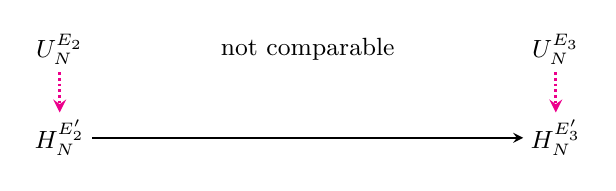
\begin{tikzpicture}[x=1cm,y=1cm,>=stealth,inner sep=2.5pt,font=\small]
\node (u2) at (0,1.12) {$U_N^{E_2}$};
\node (u3) at (6.3,1.12) {$U_N^{E_3}$};
\node at (3.15,1.12) {not comparable};
\node (h2) at (0,0) {$H_N^{E_2'}$};
\node (h3) at (6.3,0) {$H_N^{E_3'}$};
\draw[->,line width=.6pt] (h2) -- (h3);
\foreach \a/\b in {u2/h2,u3/h3}
  \draw[->,densely dotted,magenta,line width=1.05pt] (\a.south) -- (\b.north);
\end{tikzpicture}
\caption{An extra inclusion in the image of the correspondence.}
\label{extra-order-picture}
\end{figure}

It is also instructive to see what happens if we try to encode $D$ in a simpler way, by using powers. Consider the group $R_N^D$ generated by reflections $g_1,\ldots,g_N$, with the relations $(g_ig_j)^{2k}=1$, for any $i,j$ and any $k\in D$. If $d$ is the greatest common divisor of the elements of $D$ then, by the B\'ezout theorem, these relations reduce to $(g_ig_j)^{2d}=1$. Thus this construction only remembers $d$, and for instance it cannot distinguish between $\{0,2,3,4,\ldots\}$ and $\mathbb N_0$.

Let us look now at the unitary half-liberations. With $K=\{1,2,3,\ldots\}$ and $Q=\{2,3,4,\ldots\}$ we have $U_N^K=U_N^\times$ and $U_N^Q=U_N^{**}$, as explained in Section~\ref{unitary}. The allowed crossing distances are respectively $0$, and $0,1$. On the reflection side, these parameters are obtained from $\mathbb N_0$ and from $D_*$ by removing $0$, which amounts in doubling the standard reflections. Recall also that $H_N^*\subset H_N^+$ is the quantum group obtained by imposing the half-commutation relations $uvw=wvu$ to the standard coordinates. See \cite{bcs}.

\begin{thm}\label{half-pairs}
The reflection partner of $U_N^\times$ is the half-liberation $H_N^*$, and we have
\[
 H_N^*=U_N^\times\cap H_N^+.
\]
The reflection partner of $U_N^{**}$ is generated by $H_N$ and by the diagonal group duals coming from the doubled path. The largest dimensions where these partners have free diagonals are $2$ and $4$, respectively.
\end{thm}

\begin{proof}
For $K$ we have $W_K=\mathbb Z_2*\mathbb Z_2$, with standard reflections $s,s'$. Given a choice $r_1,\ldots,r_N\in\{s,s'\}$, among any 3 of these reflections, 2 are equal. Thus we have $r_ir_jr_k=r_kr_jr_i$ for any $i,j,k$, and so the generators of $K'[N]$ satisfy the half-commutation relations $g_ig_jg_k=g_kg_jg_i$. We claim that there are no other relations. Consider indeed the group $L$ generated by reflections $g_1,\ldots,g_N$, with the half-commutation relations. With $h=g_1$ and $z_i=g_ih$, the half-commutation relations tell us that
\[
 z_iz_j=z_jz_i,\qquad hz_ih=z_i^{-1}.
\]

Thus any element of $L$ can be written as follows, with $v_i\in\mathbb Z$ and $e\in\{0,1\}$:
\[
 z_2^{v_2}\ldots z_N^{v_N}h^e.
\]

Assume that such an element is killed by all the choices as above. With $r_i=s$ for any $i$ we obtain $s^e=1$, so $e=0$. Then, with $r_i=s'$ and $r_j=s$ for $j\neq i$ we obtain $(s's)^{v_i}=1$, so $v_i=0$. Thus our element is trivial, and $K'[N]=L$.

On the other hand in $H_N^*$ the squares of the coordinates are central, as we can see by taking $u=v$ in the half-commutation relations. Thus, according to \cite{rw}, we have $H_N^*\subset H_N^{[\infty]}$, and $H_N^*$ is determined by the dual of its diagonal torus, which is the above group $L$. We conclude that the partner of $U_N^\times$ is $H_N^*$. Regarding now the intersection formula, this follows from the fact that the coordinates of $H_N^+$ are self-adjoint, so the relations $uv^*w=wv^*u$ become $uvw=wvu$.

For $Q$ we have 2 standard reflections at each height, with reflections at different heights $i\neq j$ commuting when $|i-j|\geq2$. This is the doubled path from Figure~\ref{double-picture}, and the result follows from Theorem~\ref{generation}. The last assertion follows from Theorem~\ref{dimension}.
\end{proof}

These examples explain the need for a third coordinate in Theorem~\ref{intro-torus}. In dimension 2 the diagonal tori of $U_2^\times$ and $U_2^+$ are both duals of the free group $F_2$. However, the diagonal tori of their partners $H_2^*$ and $H_2$ are the duals of $\mathbb Z_2*\mathbb Z_2$ and of $\mathbb Z_2\times\mathbb Z_2$.

Observe also that in the above proof the convention regarding $1\in K$ is essential. If we had used 2 heights, we would have obtained a choice of type $r_1=s_0,r_2=s_0',r_3=s_1$, with $r_3$ commuting with the free reflections $r_1,r_2$, and here the half-commutation relations fail.

As a last comment, the following checks were performed by computer, with direct enumerations. For 2 to 10 points, all the $2\,226$ balanced paired rows were enumerated and, for every subset of the height differences occurring on a row, it was checked whether all the words coming from labelings with 3 labels reduce to the identity, under the prescribed commutation relations. The result agreed with the crossing test, in all the $12\,708$ cases. Also, for the $27$ sets of gaps contained in $\{1,\ldots,7\}$, with $d\leq3$ and $t=1,2$, the largest sets of pairwise free reflections at the heights $0,\ldots,23$ had $tm$ elements, and the inclusion of Theorem~\ref{torus-partner} was confirmed for all the $5\,907$ comparable pairs of parameters.

\section{Separation of reflection partners}\label{separation}

We know from Theorem~\ref{main} that 2 different parameters can be distinguished by their reflection partners, in some finite dimension. In this section we discuss the first such dimension. Let us start with the following definition:

\begin{defn}\label{first-dimension}
Given nonempty additive semigroups $D\neq E$, we denote by $n(D,E)$ the smallest integer $N$ such that $H_N^{D'}\neq H_N^{E'}$.
\end{defn}

Observe that the quantum groups $H_N^{D'}$ and $H_N^{E'}$ are different for any $N\geq n(D,E)$, because $D'[N]$ is the subgroup of $D'[N+1]$ generated by the first $N$ generators. We already know from Theorem~\ref{dimension} that for $E=\{0\}$ we have $n(D,E)=tm+1$. In general, the question can be reformulated in terms of graphs, as follows:

\begin{prop}\label{criteria}
Let $D\neq E$ be nonempty additive semigroups.
\begin{enumerate}
\item If a connected graph with $n$ vertices fits in exactly one of the graphs $X_D,X_E$, then $n(D,E)\leq n$.

\item If each graph with at most $n$ vertices, connected or not, fits in both graphs $X_D,X_E$, or in none of them, then $n(D,E)>n$.
\end{enumerate}
\end{prop}

\begin{proof}
(1) This follows from Theorem~\ref{test}.

(2) Let $w$ be a word in $g_1,\ldots,g_n$ which is a relation of $E'[n]$, and let $r_1,\ldots,r_n$ be standard reflections of $W_D$. The distinct reflections among them form a graph with at most $n$ vertices, which by assumption fits in $X_E$. As in the proof of Theorem~\ref{order}, we obtain standard reflections $\rho_1,\ldots,\rho_n$ of $W_E$ and a quotient map as follows, given by $\rho_i\to r_i$:
\[
 \langle\rho_1,\ldots,\rho_n\rangle\to\langle r_1,\ldots,r_n\rangle.
\]

Thus $w(r_1,\ldots,r_n)=1$, and so $w$ is a relation of $D'[n]$. By symmetry, $D'[n]=E'[n]$.
\end{proof}

As a first illustration, here is a family of parameters where the answer is exact. On the unitary side, these parameters are distinguished by the first translate $x_k$ which commutes with $x_0$ for one parameter, and not for the other one, as in Theorem~\ref{torus}.

\begin{thm}\label{separation-thm}
Consider the semigroups $S_q=\langle 2,2q+1\rangle=\{0,2,4,\ldots,2q,2q+1,2q+2,\ldots\}$, with $q\geq1$. For $q<r$ we have
\[
 H_N^{S_q'}=H_N^{S_r'}\iff N\leq 2q+1.
\]
Thus $n(S_q,S_r)=2q+2$, while the first translate distinguishing the unitary tori is $x_{2q+1}$.
\end{thm}

\begin{proof}
The gaps of $S_q$ are the odd numbers $1,3,\ldots,2q-1$. Thus, 2 standard reflections are free when the difference between their heights is odd, and at most $2q-1$ in absolute value.

Let $N\leq2q+1$, and consider a choice $r_1,\ldots,r_N$ of standard reflections. The reflections at even heights commute, and so do those at odd heights. Thus, if $I\subset\{1,\ldots,N\}$ is the set of indices of the reflections at even heights, the group $\langle r_1,\ldots,r_N\rangle$ is a quotient of the free product of $\mathbb Z_2^I$ with $\mathbb Z_2^{I^c}$. We claim that, conversely, each such free product comes from a choice. This is clear when $I$ or its complement is empty. Otherwise, with $a=|I|$, put the reflections with indices in $I$ at the heights $0,2,\ldots,2(a-1)$. The odd heights $h$ which are at distance at most $2q-1$ from all these heights are those satisfying
\[
 2(a-1)-(2q-1)\leq h\leq2q-1
\]
and there are $2q+1-a\geq N-a$ of them. Thus we have enough room for the remaining reflections. The conclusion is that for $N\leq2q+1$ the relations of the diagonal group are those which hold in all the free products of the above type, independently of $q$.

In dimension $N=2q+2$, observe that each standard reflection for $S_q$ is free from exactly $2q$ other standard reflections. Thus the graph formed by a vertex joined to $2q+1$ other vertices fits in $X_{S_r}$, but not in $X_{S_q}$, and Proposition~\ref{criteria} applies. Finally, the assertion about the unitary side follows from Theorem~\ref{torus}, because $2q+1$ is the first integer which is a gap for $S_r$, but not for $S_q$.
\end{proof}

At $q=1$, $r=2$ the 2 parameters are $\langle2,3\rangle=D_*$ and $\langle2,5\rangle$. In dimension 3 both reflection partners are generated by $H_3$ and by the diagonal dual of $(\mathbb Z_2\times\mathbb Z_2)*\mathbb Z_2$. In dimension 4 the partner of $\langle2,5\rangle$ contains in addition the diagonal dual of $\mathbb Z_2*\mathbb Z_2^3$, coming from the reflection at $0$ and those at $-1,1,3$.

\begin{figure}[H]\centering
\begin{tikzpicture}[x=1cm,y=1cm,thick]
\draw (-1,0)--(0,0)--(1,0);
\foreach \x in {-1,0,1}{\fill (\x,0) circle(2.5pt);\node[below] at (\x,-.08){$\x$};}
\begin{scope}[shift={(5,0)}]
\draw (0,0)--(-1.1,.8) (0,0)--(0,-.85) (0,0)--(1.1,.8);
\foreach \x/\y in {0/0,-1.1/.8,0/-.85,1.1/.8}\fill (\x,\y) circle(2.5pt);
\node[right] at (.12,-.08){$0$};\node[above] at (-1.1,.8){$-1$};
\node[below] at (0,-.87){$1$};\node[above] at (1.1,.8){$3$};
\end{scope}
\end{tikzpicture}
\caption{For $\langle2,5\rangle$ the reflection at $0$ is free from those at $-1,1,3$. For $\langle2,3\rangle$ it is only free from those at $-1,1$. This distinguishes the partners in dimension 4.}
\label{four-star}
\end{figure}

Let us discuss now the general case. We restrict the attention to the parameters which are numerical semigroups, as in Section~\ref{recover}. Given such a semigroup $S$, we denote by $m_S$ its smallest positive element, and by $\gamma_S$ the number of its gaps. Recall from Section~\ref{recover} that the graph $X_S$ is the graph $Y_B$, with $B$ being the set of gaps of $S$.

\begin{thm}\label{separation-general}
Let $S\neq T$ be numerical semigroups, and let $g$ be the largest gap of $S$ or $T$.
\begin{enumerate}
\item If $m_S\neq m_T$ then $n(S,T)=\min(m_S,m_T)+1$.

\item If $\gamma_S\neq\gamma_T$ then $n(S,T)\leq2\min(\gamma_S,\gamma_T)+2$.

\item In general, we have $n(S,T)\leq2g^3$.
\end{enumerate}
\end{thm}

\begin{proof}
(1) This follows from Theorem~\ref{dimension}, because for $N\leq\min(m_S,m_T)$ both partners are equal to $H_N^{[\infty]}$, and in the next dimension only one of them is.

(2) Each vertex of $X_S$ has $2\gamma_S$ neighbors, and similarly for $T$. Thus, if $\gamma_S<\gamma_T$, the graph formed by a vertex joined to $2\gamma_S+1$ other vertices fits in $X_T$, but not in $X_S$.

(3) When $\gamma_S\neq\gamma_T$ this follows from (2), because the smallest of these numbers is at most $g-1$. So, assume $\gamma_S=\gamma_T=\gamma$. Then $\gamma\leq g-1$ and $g\geq2$. Let $F$ be the ball of radius $\gamma g+1$ around $0$ in $X_S$. If $F$ fits in $X_T$ then, up to a translation, by Lemma~\ref{balls} the balls of radius $\gamma g$ around $0$ are isomorphic, and by Lemma~\ref{steps} we obtain $S=T$, contradiction. Thus $F$ does not fit in $X_T$, and since $F$ is connected, Proposition~\ref{criteria} applies. Finally, the vertices of $F$ are integers of absolute value at most $(\gamma g+1)g$, so their number is at most
\[
 2(\gamma g+1)g+1\leq2(g^2-g+1)g+1\leq2g^3
\]
and we are done.
\end{proof}

The above general bound is certainly far from being optimal. Let $k$ be the smallest integer which belongs to exactly one of the semigroups $S,T$. This is the index of the first translate $x_k$ distinguishing the unitary tori, and it is quite natural to expect that the reflection partners can be distinguished by looking at the reflections at the heights $0,1,\ldots,k$. In small cases, this can be checked by using a computer:

\begin{thm}\label{separation-computer}
Let $S\neq T$ be numerical semigroups whose gaps are all at most $12$, and let $k$ be the smallest integer which belongs to exactly one of them. Then
\[
 n(S,T)\leq k+1
\]
and in particular $n(S,T)\leq g+1$, with $g$ being the largest gap of $S$ or $T$. This latter bound is optimal, for any $g$.
\end{thm}

\begin{proof}
Assume that $k$ is a gap of $S$, and consider the graph $F$ formed by the heights $0,1,\ldots,k$, with 2 heights being joined when their difference is a gap of $S$. This graph is connected, because $1$ is a gap of $S$, and it fits in $X_S$. The program \texttt{dimension.cpp} checks, by an exhaustive search, that $F$ does not fit in $X_T$, for all the $14\,535$ pairs in the statement. Thus Proposition~\ref{criteria} applies. Regarding the last assertion, the semigroups $\{0,g,g+1,\ldots\}$ and $\{0,g+1,g+2,\ldots\}$ have largest gap $g$, and by Theorem~\ref{separation-general} (1) we have $n=g+1$ for them.
\end{proof}

Observe that $n(S,T)=k+1$ holds as well for the semigroups in Theorem~\ref{separation-thm}. We believe that the above bound holds in general, and in fact that the reason behind it is a quite simple one, namely that the graph $F$ in the above proof has too many edges for fitting in $X_T$. To be more precise, our first conjecture is as follows:

\begin{conjecture}\label{conj-separation}
For any numerical semigroups $S\neq T$ we have $n(S,T)\leq k+1$, with $k$ being the smallest integer which belongs to exactly one of them. In particular, the largest possible value of $n(S,T)$, for semigroups having all gaps at most $g$, is $g+1$.
\end{conjecture}

Regarding now the reason behind this, the statement that we have in mind, which no longer involves quantum groups, is as follows:

\begin{conjecture}\label{conj-edges}
Let $B$ be the set of gaps of a numerical semigroup. Then any set of $n$ integers contains at most
\[
 \sum_{b\in B,\,b<n}(n-b)
\]
pairs of elements whose difference is a gap, this being the number of such pairs for $n$ consecutive integers.
\end{conjecture}

In other words, the second conjecture states that in the graph $Y_B$, the sets of $n$ consecutive integers span the largest possible number of edges, among the sets with $n$ elements. Equivalently, these are the sets having the smallest number of edges leaving the set. Observe that such a statement fails for arbitrary finite sets $B$. For instance with $B=\{1,4\}$ the set $\{0,1,4,5\}$ contains 4 pairs with difference in $B$, while $\{0,1,2,3\}$ contains only 3 such pairs. Thus, the semigroup property must be used.

\begin{prop}
Conjecture~\ref{conj-edges} implies Conjecture~\ref{conj-separation}.
\end{prop}

\begin{proof}
Let $F$ be as in the proof of Theorem~\ref{separation-computer}. The integers smaller than $k$ are gaps for both semigroups or for none, and $k$ is a gap only for $S$. Thus the number of edges of $F$ is one more than the number of pairs in $\{0,\ldots,k\}$ whose difference is a gap of $T$. If Conjecture~\ref{conj-edges} holds for $T$, with $n=k+1$, the graph $F$ has too many edges for fitting in $X_T$.
\end{proof}

We have verified Conjecture~\ref{conj-edges} for all the numerical semigroups having gaps at most $9$, and for all the subsets of $\{0,\ldots,18\}$, with the program \texttt{isoperimetry.py}. In terms of the order from Section~\ref{examples}, the statement is that $n$ consecutive integers have the smallest possible number of comparable pairs, among the sets of $n$ integers. Finally, let us mention that, according to Proposition~\ref{criteria}, a lower bound for $n(S,T)$ requires looking at all the small graphs fitting in $X_S,X_T$. We do not know if $n(S,T)$ has a simple formula.

\section{Generating the free unitary group}\label{joint-section}

We have constructed the reflection partner $H_N^{D'}$ inside $H_N^+$. Let us put it now beside $U_N^D$, inside $U_N^+$. What do these 2 subgroups generate together? As a piece of motivation here, it is known from \cite{chir} that $U_N$ and $U_{N-1}^+$ generate $U_N^+$, at any $N\geq3$. In our setting we will only need 2 free reflections, acting on a coordinate plane.

Let us first look at $N=2$. With $s,t$ being the standard generators of $\mathbb Z_2*\mathbb Z_2$, consider the assignment $a\to s$, $b\to t$ on the generators of the dual of the diagonal torus of $U_2^D$. The elements $x_j=a^j(ba^{-1})a^{-j}$ are mapped in this way to $ts$ when $j$ is even, and to its inverse $st$ when $j$ is odd, and these elements commute. Thus, the relations in Theorem~\ref{torus} are satisfied, and so $U_2^D$ contains the dual of $\mathbb Z_2*\mathbb Z_2$, with fundamental representation $diag(s,t)$. Together with $S_2\subset U_2^D$, this group dual generates $H_2^{[\infty]}$, by Theorem~\ref{generation}. Thus, for any $D$, we have
\[
 H_2^{D'}\subset H_2^{[\infty]}\subset U_2^D.
\]

In particular the 2 partners generate $U_2^D$. Observe that for $0\in D$ with $D\neq\mathbb N_0$ we have $U_2^D\neq U_2^+$, because the elements $x_0,x_1$ of the diagonal torus commute, due to $1\notin D$.

Let us look now at $N\geq3$. We denote by $T_N\subset U_N^+$ the dual of the group $\mathbb Z_2*\mathbb Z_2=\langle s,t\rangle$, with fundamental representation as follows:
\[
 diag(1,s,t,1,\ldots,1).
\]

Thus, we have 2 free reflections acting on the plane spanned by $e_2,e_3$. The fixed coordinate $e_1$ will be of great use, in what follows.

\begin{prop}\label{plane-subgroup}
Let $D\neq\mathbb N_0$ be an additive semigroup containing $0$. Then $T_N\subset H_N^{D'}$, at any $N\geq3$.
\end{prop}

\begin{proof}
We have $1\notin D$, so $s_0,s_1$ are free. Consider the choice of standard reflections given by $r_2=s_0$, $r_3=s_1$, and $r_i=s_{-1}$ for $i\neq2,3$. By Lemma~\ref{retraction} we can send $s_{-1}\to1$, and we obtain a quotient map from $\langle r_1,\ldots,r_N\rangle$ onto $\mathbb Z_2*\mathbb Z_2$, which acts on the diagonal matrices as follows:
\[
 diag(s_{-1},s_0,s_1,s_{-1},\ldots,s_{-1})\to diag(1,s,t,1,\ldots,1).
\]
 Thus $T_N$ is a subgroup of the dual of $\langle r_1,\ldots,r_N\rangle$, which is in turn a subgroup of $H_N^{D'}$.
\end{proof}

In order to prove the generation result, we will compute the common fixed vectors. We will need the following independence result:

\begin{lem}\label{height-basis}
Let $D$ be an additive semigroup containing $0$, and let $\alpha$ be a colored row.
\begin{enumerate}
\item The vectors $\xi_\pi\in(\mathbb C^n)^{\otimes k}$ with $\pi\in I_D(\alpha)$ are linearly independent, at any $n\geq2$.

\item If the colors of $\alpha$ alternate, the vectors $\xi_\pi\in(\mathbb C^2)^{\otimes k}$ with $\pi$ noncrossing form a basis of the space of vectors which are fixed by $SU_2$, acting by $Q^{\otimes\alpha}$.
\end{enumerate}
\end{lem}

\begin{proof}
(1) Let us group the tensor positions according to their height. Since $0\in D$, the strings of $\pi$ at a given height do not cross, and so $\xi_\pi$ becomes a tensor product of vectors associated to noncrossing pairings, one for each height. Now the vectors associated to the noncrossing pairings of a given row are linearly independent at $n\geq2$, see \cite{bcv}, and so are their tensor products.

(2) Here $k=2j$ is even, each noncrossing pairing joins points of different colors, and so the corresponding vector is fixed. The number of noncrossing pairings is the Catalan number
\[
 C_j=\frac{1}{j+1}\binom{2j}{j}.
\]

On the other hand, the fundamental representation of $SU_2$ is equivalent to its conjugate, and by the Clebsch--Gordan rules the number of copies of the trivial representation inside its $2j$-th tensor power is the number of walks with $2j$ steps on $\mathbb N_0$, from $0$ to $0$, which is $C_j$ too. Together with the independence coming from (1), this gives the result.
\end{proof}

As an illustration for what follows, consider the pairing from Figure~\ref{pairing-walk}. Label the string $(1,4)$ by the index $2$, the string $(2,7)$ by the index $3$, and the other 2 strings by the index $1$. The corresponding basis vector appears in $\xi_\pi$, and $T_N$ multiplies it by the following word:

\begin{figure}[H]\centering
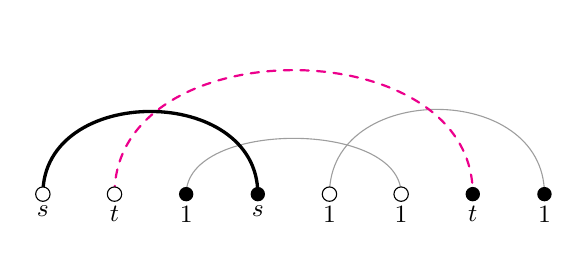
\begin{tikzpicture}[x=.91cm,y=.70cm,line cap=round,font=\small]
\draw[black!38] (3,0) .. controls (3,1.35) and (6,1.35) .. (6,0);
\draw[black!38] (5,0) .. controls (5,2.05) and (8,2.05) .. (8,0);
\draw[very thick] (1,0) .. controls (1,2) and (4,2) .. (4,0);
\draw[thick,dashed,magenta] (2,0) .. controls (2,3) and (7,3) .. (7,0);
\foreach \i in {1,2,5,6}\draw[fill=white] (\i,0) circle (2.6pt);
\foreach \i in {3,4,7,8}\fill (\i,0) circle (2.6pt);
\foreach \i/\letter in {1/s,2/t,3/1,4/s,5/1,6/1,7/t,8/1}
  \node[below] at (\i,-.04) {$\letter$};
\end{tikzpicture}
\caption{The 2 crossing strings contribute with the word $stst\neq1$. Thus, the vector associated to this pairing is not fixed by $T_N$.}
\end{figure}

Thus a crossing can be detected by $T_N$. The problem however is that a linear combination of vectors $\xi_\pi$ could be fixed, due to cancellations. In order to deal with this, we reserve the label $s$ for one string. Elsewhere we still have 2 labels, namely $1$ and $t$, and we can use the above independence results, in dimension 2. Here is the result:

\begin{thm}\label{generation-three}
Let $D\subset\mathbb N_0$ be an additive semigroup containing $0$. Then
\[
 \langle U_3^D,T_3\rangle=U_3^+
\]
where $T_3$ is the dual of $\mathbb Z_2*\mathbb Z_2=\langle s,t\rangle$, with fundamental representation $diag(1,s,t)$.
\end{thm}

\begin{proof}
Let $\alpha$ be a colored row, and consider a vector which is fixed by both $U_3^D$ and $T_3$. By Theorem~\ref{mang-weber} and Lemma~\ref{height-basis} we can write this vector in a unique way as
\[
 \xi=\sum_{\pi\in I_D(\alpha)}c_\pi\,\xi_\pi
\]
and we must prove that $c_\pi=0$, whenever $\pi$ has crossings. We proceed in several steps.

(1) Cutting along a string. Fix 2 points $p<q$ of different colors, having the same height, so that $P=(p,q)$ is a possible string. Consider the component of $\xi$ on the basis vectors having the index 2 at the positions $p,q$, and indices 1 or 3 elsewhere. Only the pairings containing $P$ contribute, because the index 2 at $p$ must be matched. By removing the 2 positions $p,q$ we obtain the following vector, in the tensor power of the space spanned by $e_1,e_3$:
\[
 \eta=\sum_{\pi\ni P}c_\pi\,\xi_{\pi-P}.
\]

(2) Using the reflections. Let $I$ be the set of positions between $p$ and $q$. The group dual $T_3$ multiplies a basis vector as above by a word of type $t^as\,t^bs\,t^c$, where $a,b,c$ are the numbers of indices equal to 3 before $p$, inside $I$, and after $q$. When $b$ is odd this word is nontrivial, and so the corresponding coefficient of $\eta$ must vanish. In other words, $\eta$ is fixed by the matrix $R=diag(1,-1)$, acting on all the positions inside $I$.

(3) Using the unitaries. Fix a height $h$, different from the height of $P$. Each $\xi_{\pi-P}$ is fixed by any matrix $Q\in U_2$ acting on all the positions of height $h$, via $Q$ at the white points, and $\bar Q$ at the black points. Indeed, each string of height $h$ joins 2 such points, of different colors. Thus $\eta$ is fixed as well. By conjugating the action from (2) by this action, and then multiplying by the action from (2) again, we conclude that $\eta$ is fixed by the matrix
\[
 QRQ^{-1}R
\]
acting on the positions of height $h$ which are inside $I$, with the same color convention. Now observe that for the following matrices, with $z=1$ or $z=i$, we have $RQR=Q^{-1}$, and so the above matrix is $Q^2$:
\[
 Q=\begin{pmatrix}\cos\theta&z\sin\theta\\-\bar z\sin\theta&\cos\theta\end{pmatrix}.
\]

By varying $\theta$ we obtain rotations about 2 different axes, which generate $SU_2$. Thus $\eta$ is fixed by $SU_2$ acting on the positions of height $h$ inside $I$, and then also by $SU_2$ acting on the positions of height $h$ outside $I$.

(4) Conclusion. Between $p$ and $q$ the walk returns to its initial level, and the same happens outside. Thus the positions of height $h$ inside $I$ have alternating colors, and so do those outside $I$. By Lemma~\ref{height-basis} (2), with respect to the positions of height $h$, the vector $\eta$ is a combination of vectors coming from noncrossing pairings which do not join the inside to the outside, with coefficients which are tensors at the other heights:
\[
 \eta=\sum_\sigma\xi_\sigma\otimes\eta_\sigma.
\]

By comparing with the formula of $\eta$ from (1), and by using the independence from Lemma~\ref{height-basis} (1), we obtain $c_\pi=0$ whenever $\pi$ contains $P$, and has a string of height $h$ which crosses $P$. By varying $h$ and $P$, and since strings of the same height cannot cross, we conclude that $c_\pi=0$ whenever $\pi$ has crossings.

Thus the common fixed vectors are those of $U_3^+$, and the result follows by Tannakian duality.
\end{proof}

We have verified the above cutting procedure, in a direct way, for all the colored rows on up to 16 points. For each row we formed the matrix having a column for each pairing with crossings, and a row for each basis vector as in the step (2), with $b$ odd, the entries being 0 or 1. For $D=\{0\}$ and for $D_*$ the columns were linearly independent, in all cases. This includes $133\,116$, respectively $126\,204$ pairings with crossings, on the $12\,870$ rows of length 16.

Finally, the same holds in any dimension $N\geq3$, the result being as follows:

\begin{thm}\label{joint-generation}
Let $D\subset\mathbb N_0$ be an additive semigroup containing $0$. Then
\[
 \big\langle U_N^D,H_N^{D'}\big\rangle=U_N^+
\]
for any $N\geq3$. When $D\neq\mathbb N_0$, the subgroup $T_N\subset H_N^{D'}$ suffices, and $N=3$ is the first dimension where the $2$ partners generate $U_N^+$.
\end{thm}

\begin{proof}
For $D=\mathbb N_0$ we have $U_N^D=U_N^+$. So, assume $D\neq\mathbb N_0$. In view of Proposition~\ref{plane-subgroup}, it is enough to prove that we have $\langle U_N^D,T_N\rangle=U_N^+$. Let $\Phi:\mathbb C^N\to\mathbb C^3$ be the projection onto the first 3 coordinates. For any pairing $\pi$ of $k$ points, we have
\[
 \Phi^{\otimes k}\xi_\pi^{(N)}=\xi_\pi^{(3)}
\]
with the upper indices standing for the dimension. Also, $\Phi$ intertwines the diagonal representations of $\mathbb Z_2*\mathbb Z_2$ in dimensions $N$ and $3$. Now consider a vector fixed by $U_N^D$ and $T_N$, written as a combination of vectors $\xi_\pi^{(N)}$ with $\pi\in I_D(\alpha)$. Its projection is the combination of the vectors $\xi_\pi^{(3)}$ with the same coefficients, which is fixed by $U_3^D$ and by $T_3$. By Theorem~\ref{generation-three} and by Lemma~\ref{height-basis} (1), the coefficients of the pairings having crossings vanish. Thus our vector is fixed by $U_N^+$, and we are done. The last assertion follows from the above discussion at $N=2$.
\end{proof}

This proves Theorem~\ref{intro-joint}. Regarding the case $0\notin D$, the situation is different for the half-liberation $U_N^\times$. Indeed, by Theorem~\ref{half-pairs} its partner $H_N^*$ is contained in $U_N^\times$, and so the 2 partners generate $U_N^\times$:
\[
 \big\langle U_N^\times,H_N^*\big\rangle=U_N^\times.
\]

For the other parameters we still have $T_N\subset H_N^{D'}$, by the same proof as for Proposition~\ref{plane-subgroup}, and the vector associated to the pairing $(1,4),(2,5),(3,6)$ from Section~\ref{tori} is not fixed by $T_N$. However, the above method does not apply, because Lemma~\ref{height-basis} fails for $0\notin D$. Thus, we are led to the question of knowing whether the quantum groups $U_N^D$ and $H_N^{D'}$ generate $U_N^+$, for $N$ big enough, when $D$ is a nonempty additive semigroup with $0,1\notin D$. We do not know the answer.

\section{Reflection character laws}\label{reflection-laws}

We discuss now the main characters of our quantum groups, with respect to the Haar integration. In this section we look at the reflection side. The computation works in fact for any quantum group $H_N^\Gamma$ as in Section~\ref{reflection}, so let $\Gamma=\langle g_1,g_2,\ldots\rangle$ be as there, with $\Gamma_N=\langle g_1,\ldots,g_N\rangle$. Recall that the main character is $\chi_N=\sum_iu_{ii}$.

\begin{thm}\label{poisson-reflections}
Let $f$ be a Poisson variable of parameter $1$, independent from the group algebra of $\Gamma$, which is taken with its canonical trace. With $N\to\infty$, the main character of $H_N^\Gamma$ converges in law, and in moments, to the variable
\[
 Y=g_1+\ldots+g_f
\]
with the convention that the empty sum is $0$. Equivalently, the limiting law is the average of the laws of the variables $g_1+\ldots+g_m$, with the Poisson weights $e^{-1}/m!$.
\end{thm}

\begin{proof}
We have $u_{ij}=g_i\otimes p_{ij}$, inside $C^*(\Gamma_N)\otimes C(S_N)$. The Haar integration is the tensor product of the canonical trace of the group algebra with the uniform integration over $S_N$. Indeed, by applying the comultiplication to a group element tensor a function on $S_N$, on each pair of permutations we obtain the group element on the first leg, and a relabeling of it on the second leg. These are both nontrivial, unless the group element is trivial, and in this latter case the invariance reduces to that of the uniform measure on $S_N$.

Since $p_{ii}(\sigma)=1$ when $\sigma(i)=i$, and $p_{ii}(\sigma)=0$ otherwise, the main character at $\sigma$ is the sum of the generators $g_i$ over the fixed points of $\sigma$:
\[
 \chi_N(\sigma)=\sum_{\sigma(i)=i}g_i.
\]

Since the relations of $\Gamma$ are invariant under relabelings, the law of such a sum only depends on the number of terms. Thus $\chi_N$ has the law of $g_1+\ldots+g_{f_N}$, with $f_N$ being the number of fixed points of a random permutation, which converges in law to $f$. Finally, the convergence in moments follows from the fact that the norm of the sum is at most $f_N$, whose factorial moments are, for any $b\leq N$:
\[
 E\big[f_N(f_N-1)\ldots(f_N-b+1)\big]=1.
\]
\end{proof}

The moments can be computed as follows. Given a partition $\pi$ of $\{1,\ldots,k\}$, having $b$ blocks, we denote by $w_\pi$ the word of length $k$ in the generators $g_1,\ldots,g_b$ obtained by labeling the blocks of $\pi$, in the order of their first elements. For instance the partition $\{1,3\},\{2,4\}$ gives $g_1g_2g_1g_2$. Now when expanding a power of $g_1+\ldots+g_m$, the words having the same pattern of equal letters as $w_\pi$ are $m(m-1)\ldots(m-b+1)$ in number, and all have the same trace. By the above formula of the factorial moments we obtain, with $h_N$ being the Haar integration,
\[
 h_N(\chi_N^k)=\#\Big\{\pi\in P(k)\ \Big|\ \pi\text{ has at most }N\text{ blocks},\ w_\pi=1\text{ in }\Gamma\Big\}.
\]

In particular the moment of order $k$ no longer depends on $N$, once $N\geq k$, and in the limit it counts the partitions $\pi\in P(k)$ with $w_\pi=1$. For our reflection partners, this leads to a formula for the free cumulants \cite{ns,free-cumulants}. Let us call a partition $\pi\in P(k)$ connected when its blocks cannot be split into 2 nonempty families, without crossings between blocks of different families. Equivalently, the only noncrossing partition which is coarser than $\pi$ is the partition having only one block.

\begin{prop}\label{cumulants}
For any nonempty additive semigroup $D$, the free cumulants of the limiting main character $Y_D$ of $H_N^{D'}$ are given by
\[
 \kappa_k(Y_D)=\#\Big\{\pi\in P(k)\ \Big|\ \pi\text{ connected},\ w_\pi=1\text{ in }D'\Big\}
\]
and in particular are positive integers, in even degrees.
\end{prop}

\begin{proof}
Assume first $1\notin D$, so that $W_D$ has infinitely many standard reflections. Consider a word of the following type, with the letters appearing in $v$ being different from those appearing in $u,u'$:
\[
 w=uvu'.
\]

We claim that $w$ is a relation of $D'$ precisely when both $v$ and $uu'$ are. One implication is clear. Conversely, assume that $w$ is a relation, and consider a choice of standard reflections for the letters of $v$. We can assign to the letters of $u,u'$ standard reflections which were not used, and then send these reflections to $1$, by using Lemma~\ref{retraction}. Since $w$ is killed, so is $v$. The proof for $uu'$ is similar. When $1\in D$ the claim holds as well. Indeed, for $D=\mathbb N_0$ the relations are the words where each letter appears an even number of times, and for $D=\{1,2,3,\ldots\}$ they are, according to the proof of Theorem~\ref{half-pairs}, the words where each letter appears as many times at odd positions as at even positions.

Now let $\pi\in P(k)$, and let $\sigma$ be the finest noncrossing partition which is coarser than $\pi$. Some block of $\sigma$ is an interval, and by using the above claim, and an induction, we conclude that $w_\pi$ is a relation precisely when all the words associated to the restrictions of $\pi$ to the blocks of $\sigma$ are relations. These restrictions are connected partitions. Thus, with $\kappa_k$ being the numbers in the statement, the moments of $Y_D$ are given by
\[
 \tau(Y_D^k)=\sum_{\sigma\in NC(k)}\ \prod_{V\in\sigma}\kappa_{|V|}
\]
and by the moment-cumulant formula \cite{ns,free-cumulants}, the numbers $\kappa_k$ are the free cumulants.
\end{proof}

As a first example, for the classical group $H_N$ the generators $g_i$ are commuting signs, and the limiting law is that of a difference of 2 independent Poisson variables of parameter $1/2$, with characteristic function $\exp(\cos x-1)$. The even moments are $1,4,31,379,\ldots$, and the free cumulants of even order, counting the connected partitions with even blocks, are $1,2,14,181,\ldots$ For $H_N^*$ the relations were described in the above proof, and the even moments are $1,3,16,131,\ldots$ These numbers, and the above formula for the free cumulants, can be checked with the program \texttt{cumulants.py}.

Let us look now at $H_N^{[\infty]}$, where the generators $g_i$ are free. We denote by $\mu_\infty$ the limiting law. Given $f=m$, the moments of $g_1+\ldots+g_m$ count the closed walks on the Cayley graph of $\mathbb Z_2^{*m}$, which is the regular tree of degree $m$. Consider a closed walk of length $2j$. Its distance to the origin is a path which stays in $\mathbb N_0$, and if it returns $r$ times to $0$, there are $m$ choices for each of the $r$ steps starting at the origin, and $m-1$ choices for each of the other $j-r$ steps going away from the origin. The number of such distance paths is known to be $\frac{r}{2j-r}\binom{2j-r}{j}$, and we obtain
\[
 \int x^{2j}\,d\mu_\infty(x)=\sum_{r=1}^j\frac{r}{2j-r}\binom{2j-r}{j}\,E\big[f^r(f-1)^{j-r}\big].
\]

The even moments are $1,3,15,105,933,9988,\ldots$ The odd moments vanish, as for any reflection partner, and the free cumulants of even order are $1,1,4,27,\ldots$

Consider now the path $D_*=\{0,2,3,\ldots\}$, and let $\mu_*$ be the corresponding limiting law. Any word which is trivial for free reflections is a relation of $D_*'$, so the moments of $\mu_*$ are at least those of $\mu_\infty$. In order to find the first moment which is different, we need the shortest word which is a relation of $D_*'$, but is nontrivial for free reflections, on any number of letters.

\begin{lem}\label{shortest-path-word}
A shortest word which is a relation of $D_*'$, but is nontrivial for free reflections, has no equal adjacent letters, including the first and last one. Each letter appears an even number of times, at least $4$. Deleting all the occurrences of a letter gives a word which is trivial for free reflections.
\end{lem}

\begin{proof}
The first assertion is clear, because a cancellation or a conjugation would produce a shorter word with the same properties. Each letter appears an even number of times, because relations hold for commuting signs. Also, as in the proof of Proposition~\ref{cumulants}, by assigning to a given letter a reflection which is not used by the other letters, and then sending this reflection to $1$, we see that deleting a letter gives a relation, which by minimality is trivial for free reflections.

Assume now that a letter $a$ appears only twice. Up to a cyclic permutation, our word is $avaz$, with $v,z$ being nonempty reduced words without $a$. Fix a choice of standard reflections for the other letters. By assigning to $a$ a reflection $s_i$ which is far away, and so commutes with the other reflections used, we obtain $vz=1$. Thus, with $v$ standing now for the corresponding element of $W_{D_*}$, for any $i\in\mathbb Z$ we have
\[
 s_ivs_iz=1\implies s_ivs_i=z^{-1}=v.
\]
 But this group has trivial center. Indeed, if $i$ is the greatest height of a reflection in the support of an element, conjugating by $s_{i+1}$ changes the support, by Lemma~\ref{retraction}. Thus $v$ is a relation of $D_*'$, and being shorter and nontrivial for free reflections, this contradicts the minimality.
\end{proof}

Here is now a word having the above properties. Consider the permutation $\sigma$ of the letters $a,b,c$ given by $a\to c\to b\to a$, and set
\[
 u=abacababcb,\qquad w=u\,\sigma(u)\,\sigma^2(u).
\]

The word $w$ has length 30, and has no equal adjacent letters. For any choice of standard reflections on the path, 2 of the 3 reflections commute, or coincide. If $a,b$ commute then the 3 parts of $w$ reduce respectively to $1$, $cacbcacb$ and $bcacbcac$, with the last 2 words being inverse to each other. Since $\sigma$ permutes cyclically the 3 parts of $w$, the same happens when another pair commutes. Thus $w$ is a relation of $D_*'$.

\begin{figure}[H]\centering
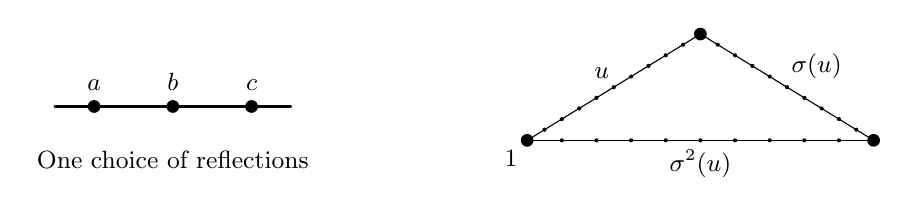
\begin{tikzpicture}[x=1cm,y=1cm,line cap=round,font=\small]
\begin{scope}
\draw[thick] (-.5,0)--(2.5,0);
\foreach \i/\j in {0/a,1/b,2/c}{\fill (\i,0) circle (2.3pt);\node[above] at (\i,.08){$\j$};}
\node at (1,-.68) {One choice of reflections};
\end{scope}
\begin{scope}[shift={(5.5,.05)}]
\coordinate (A) at (0,-.48);\coordinate (B) at (2.2,.87);\coordinate (C) at (4.4,-.48);
\foreach \a/\b in {A/B,B/C,C/A}{
  \draw (\a)--(\b);
  \foreach \j in {1,...,9}{\path (\a) -- (\b) coordinate[pos={\j/10}] (dot);\fill (dot) circle(.75pt);}
}
\foreach \a in {A,B,C}\fill (\a) circle (2.3pt);
\node[above left,inner sep=1.5pt] at (1.1,.24) {$u$};
\node[above right,inner sep=1.5pt] at (3.3,.24) {$\sigma(u)$};
\node[below] at (2.2,-.48) {$\sigma^2(u)$};
\node[below left] at (0,-.48) {$1$};
\end{scope}
\end{tikzpicture}
\caption{The word $w$ gives a closed walk of length 30 on the Cayley graph of the group generated by the first 3 generators of $D_*'$. Each side represents 10 steps.}
\end{figure}

It remains to show that this is a shortest word of this type, even when using more than 3 letters. This was done by computer, with the program \texttt{path-moments.cpp}, as follows:

\begin{prop}\label{path-census}
Up to length $30$, the only nonempty words without equal adjacent letters which are relations of $D_*'$ have length $30$, and use $3$ letters. Up to relabeling the letters, there are $10$ such words, namely the cyclic permutations of $w$.
\end{prop}

\begin{proof}
With 1 or 2 letters there are no such words, because 2 neighbors on the path are free. With 3 letters, any pair of letters can be made to commute, with the remaining letter being free from both, by using 3 consecutive heights. Thus a word in 3 letters is a relation precisely when it is trivial in each of the 3 quotients $(\mathbb Z_2\times\mathbb Z_2)*\mathbb Z_2$ of $P_3$.

Now split a word of length $2j$ as above into 2 halves, and write it as $xy^{-1}$. For each possible half, the program records its 3 reduced forms, in the 3 quotients. Different halves having the same record give a relation. For $j\leq14$ all the records are distinct. At $j=15$ the $49\,152$ halves give $60$ pairs with equal records, which are, up to the 6 relabelings of the letters, the 10 cyclic permutations of $w$.

It remains to exclude the words on more than 3 letters. By Lemma~\ref{shortest-path-word} there are at most 7 letters. Let $a$ be a letter appearing a smallest number $l$ of times, and write the word, up to a cyclic permutation, as follows:
\[
 av_1av_2\ldots av_l.
\]

For $m$ letters and length $n$, we need only consider the even numbers $l$ with $4\leq l\leq n/m$. By Lemma~\ref{shortest-path-word}, deleting $a$ gives a closed walk on the tree of the free product on the remaining letters. Inside each $v_i$ this walk first goes towards the origin, and then away from it. The program runs through the possible lengths of the words $v_i$, up to rotation and reversal, then chooses how many steps in each $v_i$ go towards the origin, and then matches each step going away from the origin with the step which undoes it. These $(n-l)/2$ matched pairs are then distributed among the other $m-1$ letters, with at least $l/2$ pairs for each letter, with adjacent letters being different.

There are 2 tests. First, for each letter $b\neq a$, mapping the other letters different from $a$ to a third letter $c$ must give a relation on 3 letters. Second, the candidates passing this first test are evaluated by putting the $m$ letters, in every order, at $m$ consecutive heights. The numbers of candidates reaching the second test, and of those passing it, are as follows:
\begin{center}
\begin{tabular}{|r|r|r|r|r|r|}
\hline
$n$ & $m=4$ & $m=5$ & $m=6$ & $m=7$ & passing \\
\hline
16 & 0 & 0 & 0 & 0 & 0\\
\hline
18 & 2 & 0 & 0 & 0 & 0\\
\hline
20 & 3 & 3 & 0 & 0 & 0\\
\hline
22 & 4 & 10 & 0 & 0 & 0\\
\hline
24 & 12 & 86 & 26 & 0 & 0\\
\hline
26 & 60 & 225 & 153 & 0 & 0\\
\hline
28 & 170 & 1184 & 1560 & 294 & 0\\
\hline
30 & 546 & 3774 & 5829 & 1748 & 0\\
\hline
\end{tabular}
\end{center}

Since words on 4 letters as in Lemma~\ref{shortest-path-word} have length at least 16, this finishes the proof.
\end{proof}

We can now compute the first moment distinguishing between the path partner and $H_N^{[\infty]}$:

\begin{thm}\label{path-moment}
Let $\mu_*$ and $\mu_\infty$ be the limiting laws of the main characters of $H_N^{D_*'}$ and $H_N^{[\infty]}$. These laws have the same moments up to order $29$, and
\[
 \int x^{30}\,d\mu_*(x)-\int x^{30}\,d\mu_\infty(x)=10
\]
with the $10$ extra contributions coming from words on $3$ letters.
\end{thm}

\begin{proof}
The moments count the partitions $\pi$ such that $w_\pi$ is a relation. A partition which contributes to $\mu_*$, but not to $\mu_\infty$, and which is of the smallest possible size, has no equal adjacent letters, because removing them would give a smaller such partition. Thus, by Proposition~\ref{path-census}, there are no such partitions up to order $29$, and exactly $10$ of them at order $30$. As for the values of the moments, the above formula for $\mu_\infty$ gives
\[
 \int x^{30}\,d\mu_\infty(x)=2\,376\,234\,441\,556\,411,\qquad\int x^{30}\,d\mu_*(x)=2\,376\,234\,441\,556\,421
\]
and we are done.
\end{proof}

\section{Unitary character laws}\label{unitary-laws}

On the unitary side the main character $\chi_N=\sum_iu_{ii}$ is no longer self-adjoint, so we must look at its $*$-moments, which are the Haar integrals of the words in $\chi_N,\chi_N^*$. Such a word corresponds to a colored row, with $\chi_N$ at the white points and $\chi_N^*$ at the black points, and by \cite{wor} its integral is the dimension of the space of fixed vectors of the corresponding representation $u^{\otimes\alpha}$. Thus, as soon as the vectors $\xi_\pi$ are linearly independent, the $*$-moments of the main character of $U_N^D$ are the numbers $|I_D(\alpha)|$.

In order to find a model for these numbers, consider a family of variables $c_j$ indexed by the integers, in a noncommutative probability space with trace $\tau$, whose joint $*$-moments are given by the following rule. The trace of a word in the variables $c_j,c_j^*$ is the number of ways of pairing the letters, with each $c_j$ being paired with a $c_j^*$ having the same index, and with 2 strings with indices $i,j$ being allowed to cross only when $|i-j|\notin D$.

Such variables exist, and are called mixed Gaussian variables. Indeed, by writing
\[
 c_j=\frac{a_j+\mathrm{i}b_j}{\sqrt{2}}
\]
the rule becomes the Wick formula of the mixed $q$-Gaussian variables from \cite{jz,speicher-field}, for the self-adjoint variables $a_j,b_j$, with the parameters $q=0$ or $q=1$, depending on whether the crossings are forbidden or allowed. In more familiar terms, the variables $c_i,c_j$ are free when $|i-j|\in D$, and independent in the classical sense when $|i-j|\notin D$. Each $c_j$ is a circular variable when $0\in D$, and a complex Gaussian variable when $0\notin D$. See \cite{cf,mlot,sw} for such mixtures of classical and free independence, and \cite{partial} for related quantum groups.

It is instructive to compare this with the reflection side. With respect to the canonical trace of $W_D$, the standard reflections $s_j$ are symmetric signs, and $s_i,s_j$ are free when $|i-j|\notin D$, and independent in the classical sense when $|i-j|\in D$. Thus, we have here the opposite rule.

Now let $v$ be a unitary implementing the shift, $vc_jv^*=c_{j+1}$, with the trace extended by the formula $\tau(Pv^a)=0$ for $a\neq0$, for any polynomial $P$ in the variables $c_j,c_j^*$.

\begin{thm}\label{unitary-character}
For any additive semigroup $D\subset\mathbb N_0$, the main character of $U_N^D$ converges in $*$-moments, with $N\to\infty$, to the variable
\[
 Z_D=c_0v
\]
and when $0\in D$ the $*$-moments are equal to those of $Z_D$ at any $N\geq2$.
\end{thm}

\begin{proof}
Consider a word in $Z_D,Z_D^*$, and the corresponding colored row and walk. We move all the shifts to the right, as in the proof of Theorem~\ref{torus}. If the walk is at $h$, the 2 possible steps give
\[
 v^hZ_D=c_hv^{h+1},\qquad v^hZ_D^*=c_{h-1}^*v^{h-1}.
\]

Thus each point of height $h$ contributes with $c_h$ if white, and $c_h^*$ if black. If the walk does not end at $0$ a power of the shift is left, and the trace vanishes. Otherwise the trace counts the pairings between points of the same height and different colors, with 2 strings being allowed to cross only when their heights are at distance outside $D$. But these are the elements of $I_D(\alpha)$.

On the other hand, as explained above, the corresponding moment of $\chi_N$ is $|I_D(\alpha)|$ when the vectors $\xi_\pi$ are linearly independent. This is the case when $N$ is at least the number of strings, as in the proof of Proposition~\ref{order-unitary}, and when $0\in D$ and $N\geq2$, by Lemma~\ref{height-basis}.
\end{proof}

What part of $D$ can be seen on the modulus of the character? In the product $Z_DZ_D^*=c_0c_0^*$ the shift cancels, and we only see whether $0$ belongs to $D$ or not:

\begin{prop}\label{modulus-law}
The law of $Z_DZ_D^*$ is the Marchenko--Pastur law of parameter $1$ when $0\in D$, and the exponential law of parameter $1$ when $0\notin D$. In particular,
\[
 \tau\big((Z_DZ_D^*)^3\big)=5\ \text{ or }\ 6
\]
depending on whether $0\in D$ or $0\notin D$.
\end{prop}

\begin{proof}
The moment of order $p$ counts the allowed pairings of $2p$ points of alternating colors, all having height $0$. When $0\in D$ these are the noncrossing pairings, counted by the Catalan numbers $C_p$, which are the moments of the Marchenko--Pastur law \cite{ns}. When $0\notin D$ each white point can be joined to any black point, and we obtain the numbers $p!$, which are the moments of the exponential law. At $p=3$ we obtain
\[
 C_3=5,\qquad3!=6
\]
as stated.
\end{proof}

In order to see the positive distances we must climb. Consider the variables $Z_D^k(Z_D^*)^k$, where the walk goes up $k$ steps, and then comes back. In the simplest case of the path $D_*$ at $k=2$, the variables $c_0,c_1$ are independent circular variables, and from $Z_{D_*}^2=c_0c_1v^2$ we see that $Z_{D_*}^2(Z_{D_*}^*)^2$ has the law of a product of 2 independent Marchenko--Pastur variables, with moments $C_p^2$. In general, the answer involves the order $i\preceq j\iff j-i\in D$ from Section~\ref{examples}, and the lattice $NC(p)$ of noncrossing partitions of $\{1,\ldots,p\}$, ordered by refinement:

\begin{thm}\label{order-maps}
Let $D\subset\mathbb N_0$ be an additive semigroup containing $0$. For any $k,p\geq1$ we have
\[
 \tau\!\left[\bigl(Z_D^k(Z_D^*)^k\bigr)^p\right]=\#\Big\{f:\{0,\ldots,k-1\}\to NC(p)\ \Big|\ i\preceq j\implies f(i)\leq f(j)\Big\}
\]
and the same holds for the main character of $U_N^D$, at any $N\geq2$.
\end{thm}

\begin{proof}
The walk goes up $k$ steps and down $k$ steps, $p$ times. Each edge $\{i,i+1\}$ with $0\leq i\leq k-1$ is run through $2p$ times, at points that we denote, with $u$ standing for up and $d$ for down, as follows:
\[
 u_1^i<d_1^i<u_2^i<d_2^i<\ldots<u_p^i<d_p^i.
\]

By Theorem~\ref{unitary-character}, we must count the families $(\pi_0,\ldots,\pi_{k-1})$, where $\pi_i$ is a noncrossing pairing of the above $2p$ points, joining points of different colors, such that the strings of $\pi_i,\pi_j$ do not cross when $i<j$ and $j-i\in D$.

(1) Noncrossing pairings and partitions. Put the above $2p$ points on a circle. The strings of $\pi_i$ cut the disk into regions. Let us call inner arcs the $p$ arcs of the circle going from $u_a^i$ to $d_a^i$, and outer arcs the $p$ remaining arcs, which go from $d_a^i$ to $u_{a+1}^i$:
\[
 u_1^i\frown d_1^i\quad d_1^i\smile u_2^i\quad u_2^i\frown d_2^i\quad\ldots\quad u_p^i\frown d_p^i\quad d_p^i\smile u_1^i.
\]
 Each string has inner arcs on one side, and outer arcs on the other side, so each region touches arcs of only one type. We obtain a partition $\sigma_i$ of $\{1,\ldots,p\}$, by putting $a,b$ in the same block when the inner arcs number $a,b$ touch the same region. It is well-known that $\pi_i\to\sigma_i$ is a bijection between the pairings in question and $NC(p)$, see \cite{ns}. Observe also that the boundary of a region touching inner arcs consists of inner arcs alternating with strings, so the blocks of $\sigma_i$ are obtained by declaring $a,b$ to be equivalent when a string of $\pi_i$ joins the points $d_a^i$ and $u_b^i$. Here are 2 examples, at $p=3$:

\begin{figure}[H]\centering
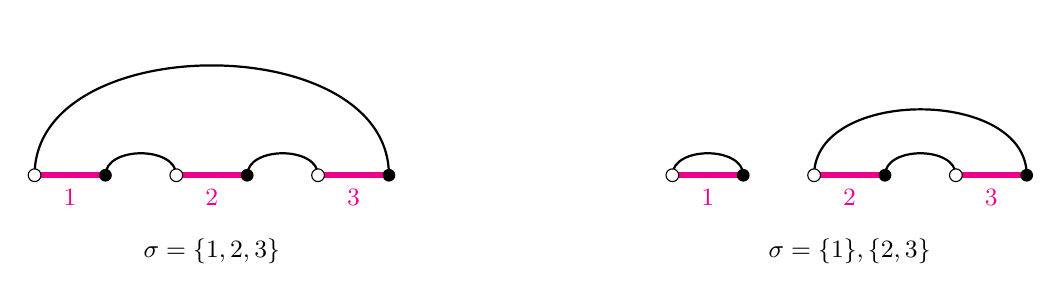
\begin{tikzpicture}[x=.9cm,y=.6cm,line cap=round,font=\small]
\foreach \offset/\pairs/\name in {0/{1/6,2/3,4/5}/{\{1,2,3\}},9/{1/2,3/6,4/5}/{\{1\},\{2,3\}}}{
 \begin{scope}[shift={(\offset,0)}]
 \foreach \a/\b in \pairs {
  \draw[thick] (\a,0) .. controls (\a,{.62*(\b-\a)}) and (\b,{.62*(\b-\a)}) .. (\b,0);}
 \foreach \a/\l in {1/1,3/2,5/3}{\draw[magenta,line width=2pt] (\a,0)--(\a+1,0);\node[below,magenta] at (\a+.5,-.1){$\l$};}
 \foreach \i in {1,3,5}{\draw[fill=white] (\i,0) circle[radius=2.3pt];}
 \foreach \i in {2,4,6}{\fill (\i,0) circle[radius=2.3pt];}
 \node at (3.5,-1.6) {$\sigma=\name$};
 \end{scope}}
\end{tikzpicture}
\caption{Noncrossing pairings of 6 points, with the points drawn on a line, and with the inner arcs in thick lines. On the left the 3 inner arcs touch the same region. On the right the first inner arc is alone, and the other 2 touch the same region.}
\label{inner-arcs}
\end{figure}

(2) The case of 2 heights. Let $i<j$. We have $u_a^i<u_a^j<d_a^j<d_a^i$ for any $a$, so the points of height $j$ lie on the inner arcs of height $i$, the points $u_a^j,d_a^j$ lying on the inner arc number $a$. A string of $\pi_j$ joining $d_a^j$ and $u_b^j$ crosses no string of $\pi_i$ precisely when its endpoints lie on inner arcs touching the same region of $\pi_i$, that is, when $a,b$ are in the same block of $\sigma_i$. By the last observation in (1), we conclude that the strings of $\pi_i,\pi_j$ do not cross precisely when each block of $\sigma_j$ is contained in a block of $\sigma_i$, that is, when $\sigma_j\leq\sigma_i$.

(3) Conclusion. We must count the maps $i\to\sigma_i$ which are decreasing with respect to $\preceq$. Since $NC(p)$ is isomorphic to its opposite, via the Kreweras complement \cite{kreweras}, their number is the number of increasing maps. The last assertion follows from Theorem~\ref{unitary-character}.
\end{proof}

We have checked the above formula with the program \texttt{orders.py}, which counts the pairings in a direct way, for several semigroups $D$. Here are some consequences:

(1) For $D=\mathbb N_0$, where the quantum group is $U_N^+$, the order $\preceq$ is the usual one, and we must count the chains $\sigma_0\leq\ldots\leq\sigma_{k-1}$ in $NC(p)$. By \cite{edelman} we obtain the Fuss--Catalan numbers
\[
 \frac{1}{kp+1}\binom{(k+1)p}{p}.
\]

(2) For $D=\{0\}$ there is no condition, and we obtain $C_p^k$. More generally, for $D=d\mathbb N_0$ the integers are comparable when they are congruent modulo $d$, and we obtain a product of $d$ Fuss--Catalan numbers.

(3) At $p=2$ the lattice $NC(2)$ has 2 elements, and an increasing map is determined by the smallest elements, with respect to $\preceq$, where it takes the largest value. These form an antichain, and any antichain can appear. Thus we obtain the number of antichains of $\{0,\ldots,k-1\}$.

This latter observation is of particular interest, in view of the discussion in Section~\ref{examples}, and holds in fact without assuming $0\in D$. Consider the numbers
\[
 A_k=\tau\!\left[\bigl(Z_D^k(Z_D^*)^k\bigr)^2\right]
\]
with the convention $A_0=1$. We have then the following result:

\begin{thm}\label{character-recovery}
For any nonempty additive semigroup $D$, the number $A_k$ counts the subsets of $\{0,\ldots,k-1\}$ whose distinct elements are at distances outside $D$. Equivalently, when $1\notin D$, the number $A_k$ counts the sets of pairwise free reflections among $s_0,\ldots,s_{k-1}$. Moreover, for any $d\geq1$ we have
\[
 d\in D\iff A_{d+1}-2A_d+A_{d-1}=0
\]
so these numbers, together with the number from Proposition~\ref{modulus-law}, determine $D$. All these numbers can be computed with the main character of $U_3^D$, which therefore determines $D$.
\end{thm}

\begin{proof}
When $0\in D$ the first assertion follows from Theorem~\ref{order-maps}, as explained above. In general, at $p=2$ each edge is run through 4 times, and exactly as in the proof of Lemma~\ref{crossing-exists}, we have 2 possible choices $P_i,Q_i$ at each height $i$, with the strings at heights $i<j$ crossing precisely when we choose $P_i$ and $Q_j$:

\begin{figure}[H]\centering
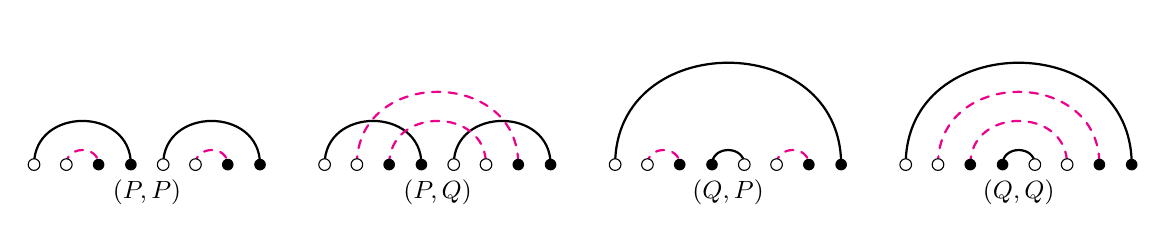
\begin{tikzpicture}[x=.41cm,y=.44cm,line cap=round,font=\small]
\foreach \offset/\loType/\hiType in {0/P/P,9/P/Q,18/Q/P,27/Q/Q}{
 \begin{scope}[shift={(\offset,0)}]
 \def\test{P}
 \ifx\loType\test \def\lowpairs{1/4,5/8}\else\def\lowpairs{1/8,4/5}\fi
 \ifx\hiType\test \def\hipairs{2/3,6/7}\else\def\hipairs{2/7,3/6}\fi
 \foreach \a/\b in \lowpairs {
  \draw[thick] (\a,0) .. controls (\a,{.56*(\b-\a)}) and (\b,{.56*(\b-\a)}) .. (\b,0);}
 \foreach \a/\b in \hipairs {
  \draw[thick,dashed,magenta] (\a,0) .. controls (\a,{.56*(\b-\a)}) and (\b,{.56*(\b-\a)}) .. (\b,0);}
 \foreach \i in {1,2,5,6}{\draw[fill=white] (\i,0) circle[radius=2.1pt];}
 \foreach \i in {3,4,7,8}{\fill (\i,0) circle[radius=2.1pt];}
 \node at (4.5,-.8) {$(\loType,\hiType)$};
 \end{scope}}
\end{tikzpicture}
\caption{The 4 choices at 2 heights, with the lower height in solid lines. Only the choice $(P,Q)$ produces crossings.}
\label{four-pairings}
\end{figure}

Thus the allowed choices are those where the set $M$ of heights carrying $Q$ has the following property:
\[
 j\in M,\ i<j,\ j-i\in D\implies i\in M.
\]

Such a set is determined by its elements $j$ having no element of $M$ at $j+D$, apart from $j$ itself, which are at distances outside $D$ from each other, and any set of heights with this latter property can appear. This gives the first assertion, and the second one is a reformulation of it.

Regarding now the formula, by inclusion-exclusion and by translation invariance, the number $A_{d+1}-2A_d+A_{d-1}$ counts the subsets as above of $\{0,\ldots,d\}$ which contain both $0$ and $d$. There are no such subsets when $d\in D$, and when $d\notin D$ the set $\{0,d\}$ is one.

Finally, the tensors associated to $P_i,Q_i$ are linearly independent in dimension 2, and so are their tensor products over the various heights. Thus the numbers $A_k$ are $*$-moments of the main character of $U_N^D$ at any $N\geq2$. As for the number from Proposition~\ref{modulus-law}, here we need $N\geq3$, in order for the 6 pairings there to give linearly independent vectors.
\end{proof}

As an example, for $D_*$ the sets in question are the empty set, the $k$ sets with one element, and the $k-1$ sets consisting of 2 neighbors. Thus $A_k=2k$, at any $k\geq1$.

\section{Comparison of the character laws}\label{paired-laws}

We have now 2 variables associated to a semigroup $D$, namely the limiting main character $Z_D$ of the quantum groups $U_N^D$, and the limiting main character $Y_D$ of the reflection partners $H_N^{D'}$. In this section we compare them. The simplest relation is as follows:

\begin{thm}\label{seven}
For any additive semigroup $D\subset\mathbb N_0$ containing $0$ we have
\[
 \tau\!\left[\bigl(Z_D^2(Z_D^*)^2\bigr)^2\right]+\tau(Y_D^4)=7
\]
with $\tau$ being the expectation with respect to the corresponding laws.
\end{thm}

\begin{proof}
The unitary moment is the number $A_2$ from Theorem~\ref{character-recovery}. It counts the empty set, the sets $\{0\}$ and $\{1\}$, and the set $\{0,1\}$ when $1\notin D$. Thus
\[
 A_2=3\ \ (1\in D),\qquad A_2=4\ \ (1\notin D).
\]

The reflection moment counts the partitions of $\{1,2,3,4\}$ whose word is a relation. Since each letter must appear an even number of times, the candidates are $aaaa$, $aabb$, $abba$, which are always relations, and $abab$. When $1\notin D$ we can choose $s_0,s_1$, which are free, and $abab$ is not a relation. When $1\in D$ we have $D=\mathbb N_0$, the reflections commute, and $abab$ is a relation. Thus
\[
 \tau(Y_D^4)=4\ \ (1\in D),\qquad\tau(Y_D^4)=3\ \ (1\notin D)
\]
and by adding we obtain $7$, in both cases.
\end{proof}

In other words, the distance $1$ is either a forbidden crossing distance, and then the reflections commute, or an allowed one, and then they are free. Each of these 2 situations contributes to exactly one of the 2 moments. When $0\notin D$ the reflections $s_0,s_0'$ are free, so the reflection moment is always $3$, and the sum is no longer constant.

More generally, Theorem~\ref{character-recovery} tells us that, when $1\notin D$, the unitary moments $A_k$ count the sets of pairwise free reflections among $s_0,\ldots,s_{k-1}$. Here is a consequence of this fact:

\begin{thm}\label{free-character-range}
Let $D\neq\{0\}$ be a nonempty additive semigroup, with smallest positive element $m$, and with $t\in\{1,2\}$ reflections at each height. For any $k\geq1$, the following are equivalent:
\begin{enumerate}
\item We have $A_k=2^k$.

\item We have $k\leq m$.

\item The conditional law of $Y_D$, given $f=tk$, is the law of a sum of $tk$ free symmetric signs.
\end{enumerate}
More generally, the conditional law of $Y_D$ given $f=n$ is the law of a sum of $n$ free symmetric signs precisely when $n\leq tm$.
\end{thm}

\begin{proof}
By Theorem~\ref{character-recovery} we have $A_k=2^k$ precisely when all the distances $1,\ldots,k-1$ are outside $D$, that is, when $k\leq m$. Regarding the last assertion, the conditional law in question is the law of $g_1+\ldots+g_n$, and by Theorem~\ref{dimension} the generators $g_1,\ldots,g_n$ of $D'$ are free precisely when $n\leq tm$. When they are not free, some nonempty word without equal adjacent letters is a relation, and so some moment of $g_1+\ldots+g_n$ is strictly bigger than in the free case. Thus the law detects the freeness, and with $n=tk$ we obtain the equivalence between (2) and (3).
\end{proof}

As an example, for $D=\{0\}$ all the 8 subsets of $\{0,1,2\}$ are allowed, while for the path $D_*$ the 2 subsets containing both $0$ and $2$ are not. Thus the unitary moment of order 12 drops from $8$ to $6$. On the reflection side the moments agree up to order 29, and the moment of order 30 increases by 10, by Theorem~\ref{path-moment}.

Let us discuss now the behavior of the 2 laws when the parameter varies. On the unitary side, for $D\subset E$ we lose pairings, and so the $*$-moments of $Z_D$ are at least those of $Z_E$. By Proposition~\ref{modulus-law} and Theorem~\ref{character-recovery}, the law of $Z_D$ determines $D$. On the reflection side, we have:

\begin{prop}\label{monotone}
Assume that $H_N^{D'}\subset H_N^{E'}$ for any $N$. Then the moments of $Y_D$ are at least those of $Y_E$, and if these $2$ variables have the same law, then $D=E$.
\end{prop}

\begin{proof}
By assumption the relations of $E'$ are relations of $D'$, and so the partitions counted by the moments of $Y_E$ are among those counted by the moments of $Y_D$. If the moments are equal then the partitions are the same. Since any word in the generators is of the form $w_\pi$, up to a relabeling of the letters, we conclude that $D'$ and $E'$ have the same relations. Thus $H_N^{D'}=H_N^{E'}$ for any $N$, and Theorem~\ref{main} gives $D=E$.
\end{proof}

This applies in particular when $E\subset D$, by Theorem~\ref{torus-partner}, and also to the series of multiples from Proposition~\ref{series}. As an interesting consequence, we have the following result:

\begin{thm}\label{universality}
For any nonempty additive semigroup $D$ with $1\notin D$, the moments of $Y_D$ up to order $29$ are those of the limiting law $\mu_\infty$ for $H_N^{[\infty]}$, and
\[
 0\leq\tau(Y_D^{30})-\int x^{30}\,d\mu_\infty(x)\leq10.
\]
Thus, apart from $H_N$ and $H_N^*$, all the reflection partners have the same moments up to order $29$.
\end{thm}

\begin{proof}
Since $1\notin D$ we have $D\subset D_*$, and so by Theorem~\ref{torus-partner} we have inclusions as follows:
\[
 H_N^{D_*'}\subset H_N^{D'}\subset H_N^{[\infty]}.
\]

Thus by Proposition~\ref{monotone} the moments of $Y_D$ are between those of $\mu_\infty$ and those of the law $\mu_*$ for the path, and the result follows from Theorem~\ref{path-moment}.
\end{proof}

Summarizing, the law of $Y_D$ distinguishes the parameters which are comparable, but for parameters which are not comparable, it cannot do so with small moments. This leads to the question of knowing whether the law of $Y_D$ determines $D$, in general. That is, we would like to know if the following holds, for any nonempty additive semigroups $D,E$:
\[
 law(Y_D)=law(Y_E)\implies D=E.
\]

We do not know the answer. By Proposition~\ref{monotone}, this question only concerns the pairs of reflection partners which are not comparable. Observe also that the moments of the main character of $H_N^{D'}$ at finite $N$ count the partitions as above having at most $N$ blocks. Thus, knowing these moments at any $N$ amounts in knowing the laws of all the sums $g_1+\ldots+g_n$, and one may ask the same question for this finer invariant. Finally, in view of Proposition~\ref{cumulants}, the question is whether the numbers of connected partitions whose words are relations of $D'$ determine $D$.

\phantomsection\addcontentsline{toc}{section}{References}
\begin{thebibliography}{99}

\bibitem{bbc} T. Banica, J. Bichon and B. Collins, The hyperoctahedral quantum group, \emph{J. Ramanujan Math. Soc.} \textbf{22} (2007), 345--384.

\bibitem{bcs} T. Banica, S. Curran and R. Speicher, Classification results for easy quantum groups, \emph{Pacific J. Math.} \textbf{247} (2010), 1--26.

\bibitem{bs} T. Banica and R. Speicher, Liberation of orthogonal Lie groups, \emph{Adv. Math.} \textbf{222} (2009), 1461--1501.

\bibitem{bcf} M. Brannan, A. Chirvasitu and A. Freslon, Topological generation and matrix models for quantum reflection groups, \emph{Adv. Math.} \textbf{363} (2020), 106982.

\bibitem{bcv} M. Brannan, B. Collins and R. Vergnioux, The Connes embedding property for quantum group von Neumann algebras, \emph{Trans. Amer. Math. Soc.} \textbf{369} (2017), 3799--3819.

\bibitem{cf} M. Caspers and P. Fima, Graph products of operator algebras, \emph{J. Noncommut. Geom.} \textbf{11} (2017), 367--411.

\bibitem{chir} A. Chirvasitu, Topological generation results for free unitary and orthogonal groups, \emph{Int. J. Math.} \textbf{31} (2020), 2050003.

\bibitem{dilworth} R.P. Dilworth, A decomposition theorem for partially ordered sets, \emph{Ann. of Math.} \textbf{51} (1950), 161--166.

\bibitem{edelman} P.H. Edelman, Chain enumeration and non-crossing partitions, \emph{Discrete Math.} \textbf{31} (1980), 171--180.

\bibitem{green} E.R. Green, Graph products of groups, Ph.D. thesis, University of Leeds (1990).

\bibitem{jz} M. Junge and Q. Zeng, Ultraproduct methods for mixed $q$-Gaussian algebras, \emph{Pacific J. Math.} \textbf{331} (2024), 99--147.

\bibitem{kreweras} G. Kreweras, Sur les partitions non crois\'ees d'un cycle, \emph{Discrete Math.} \textbf{1} (1972), 333--350.

\bibitem{cyclic} A. Mang and M. Weber, Categories of two-colored pair partitions, part I: categories indexed by cyclic groups, \emph{Ramanujan J.} \textbf{53} (2020), 181--208.

\bibitem{semi} A. Mang and M. Weber, Categories of two-colored pair partitions, part II: categories indexed by semigroups, \emph{J. Combin. Theory Ser. A} \textbf{180} (2021), 105409.

\bibitem{mlot} W. Mlotkowski, $\Lambda$-free probability, \emph{Infin. Dimens. Anal. Quantum Probab. Relat. Top.} \textbf{7} (2004), 27--41.

\bibitem{morris} D.W. Morris, J. Morris and G. Verret, Isomorphisms of Cayley graphs on nilpotent groups, \emph{New York J. Math.} \textbf{22} (2016), 453--467.

\bibitem{ns} A. Nica and R. Speicher, Lectures on the combinatorics of free probability, Cambridge Univ. Press (2006).

\bibitem{rw} S. Raum and M. Weber, Easy quantum groups and quantum subgroups of a semi-direct product quantum group, \emph{J. Noncommut. Geom.} \textbf{9} (2015), 1261--1293.

\bibitem{full} S. Raum and M. Weber, The full classification of orthogonal easy quantum groups, \emph{Comm. Math. Phys.} \textbf{341} (2016), 751--779.

\bibitem{rgs} J.C. Rosales and P.A. Garc\'ia-S\'anchez, Numerical semigroups, Springer (2009).

\bibitem{trees} J.-P. Serre, Trees, Springer (1980).

\bibitem{speicher-field} R. Speicher, Generalized statistics of macroscopic fields, \emph{Lett. Math. Phys.} \textbf{27} (1993), 97--104.

\bibitem{free-cumulants} R. Speicher, Multiplicative functions on the lattice of non-crossing partitions and free convolution, \emph{Math. Ann.} \textbf{298} (1994), 611--628.

\bibitem{partial} R. Speicher and M. Weber, Quantum groups with partial commutation relations, \emph{Indiana Univ. Math. J.} \textbf{68} (2019), 1849--1883.

\bibitem{sw} R. Speicher and J. Wysoczanski, Mixtures of classical and free independence, \emph{Arch. Math.} \textbf{107} (2016), 445--453.

\bibitem{tw} P. Tarrago and M. Weber, Unitary easy quantum groups: the free case and the group case, \emph{Int. Math. Res. Not.} \textbf{2017} (2017), 5710--5750.

\bibitem{wang} S. Wang, Free products of compact quantum groups, \emph{Comm. Math. Phys.} \textbf{167} (1995), 671--692.

\bibitem{wor} S.L. Woronowicz, Tannaka-Krein duality for compact matrix pseudogroups. Twisted SU(N) groups, \emph{Invent. Math.} \textbf{93} (1988), 35--76.

\end{thebibliography}
\end{document}
